\documentclass[12pt]{ociamthesis}  % default square logo 
%\documentclass[12pt,beltcrest]{ociamthesis} % use old belt crest logo
%\documentclass[12pt,shieldcrest]{ociamthesis} % use older shield crest logo
%load any additional packages
\usepackage{amssymb}
\usepackage{graphicx}
\usepackage{enumitem}
\usepackage{algorithm}% http://ctan.org/pkg/algorithms
\usepackage{algpseudocode}
%\usepackage{algorithm}
%\usepackage{arevmath}     % For math symbols
%\usepackage[noend]{algpseudocode}





%input macros (i.e. write your own macros file called mymacros.tex 
%and uncomment the next line)
%\include{mymacros}

\title{Hierarchical \\[1ex]Leader Election Algorithm \\[1ex]     %your thesis title,
        With Remoteness Constraint}   %note \\[1ex] is a line break in the title

\author{Mohamed Tbarka}             %your name
\college{ENSIAS}  %your college

%\renewcommand{\submittedtext}{change the default text here if needed}
\degree{Software Engineering}     %the degree
\degreedate{2019}         %the degree date

%end the preamble and start the document
\begin{document}

%this baselineskip gives sufficient line spacing for an examiner to easily
%markup the thesis with comments
\baselineskip=18pt plus1pt

%set the number of sectioning levels that get number and appear in the contents
\setcounter{secnumdepth}{3}
\setcounter{tocdepth}{3}


\maketitle                  % create a title page from the preamble info
\begin{dedication}
This thesis is dedicated to\\
my grand father\\
for inspiring me.\\
\end{dedication}        % include a dedication.tex file
\begin{acknowledgements}
I would like to thank the all library media specialists for their participation in the survey who supported my work in this way and helped me get results of better quality. I am also grateful to the members of my committee for their patience and support in overcoming numerous obstacles I have been facing through my research

I would like to thank my fellow doctoral students for their feedback, cooperation and of course friendship. In addition I would like to express my gratitude to the staff of INFRES-Telecom ParisTech for  the last minute favors.

Nevertheless, I am also grateful to the Mr Petr Kuznetsov for sharing his dissertation woes, and a glimmer of hope for post-dissertation normalcy. I am also thankful to Mrs Sanaa ElFkihi for his efficient supervising.

I would like to thank my friends for accepting nothing less than excellence from me. Last but not the least, I would like to thank my family: my parents and to my brothers and sister for supporting me spiritually throughout writing this thesis and my my life in general.
\end{acknowledgements}   % include an acknowledgements.tex file
\begin{abstract}
A hierarchical algorithm for electing a leaders' hierarchy in an asynchronous network with dynamically changing communication topology is presented including a remoteness's constraint towards each leader. The algorithm ensures that, no matter what pattern of topology changes occur, if topology changes cease, then eventually every connected component contains a unique leaders' hierarchy. The algorithm combines ideas from the Temporally Ordered Routing Algorithm (TORA) for mobile ad hoc networks with a wave algorithm, all within the framework of a height-based mechanism for reversing the logical direction of communication links. Moreover, an improvement from the algorithm in is the introduction of logical clocks as the nodes’ measure of time, instead of requiring them to have access to a common global time. This new feature makes the algorithm much more flexible and applicable to real situations, while still providing a correctness proof. It is also proved that in certain well behaved situations, a new leader is not elected unnecessarily.
\end{abstract}


\newpage

\renewcommand{\abstractname}{Résumé}

\begin{abstract}
Un algorithme hiérarchique pour l'élection d'une hiérarchie de "leaders" dans un réseau asynchrone avec une topologie de communication en évolution dynamique est présenté, incluant une contrainte d'éloignement vis-à-vis de chaque leader. L'algorithme garantit que, quel que soit le modèle de modification de la topologie utilisé, si cette modification cesse, tous les composants connectés contiennent m hiérarchie de leaders unique. L'algorithme combine des idées de l'algorithme TORA (Temporally Ordered Algorithm) pour les réseaux ad hoc mobiles avec un algorithme d'onde, le tout dans le cadre d'un mécanisme basé sur la hauteur destiné à inverser le sens logique des liaisons de communication. De plus, une amélioration de l’algorithme est l’introduction d’horloges logiques comme mesure du temps des noeuds, au lieu de leur demander d’avoir accès à une heure globale commune. Cette nouvelle fonctionnalité rend l'algorithme beaucoup plus flexible et applicable à des situations réelles, tout en fournissant une preuve de correction. Il est également prouvé que dans certaines situations bien conduites, un nouveau "leader" n’est pas élu inutilement.

\end{abstract}


          % include the abstract

\begin{romanpages}          % start roman page numbering
\tableofcontents            % generate and include a table of contents
\listoffigures              % generate and include a list of figures
\end{romanpages}            % end roman page numbering

%now include the files of latex for each of the chapters etc
\chapter{Introduction}
\paragraph{}Leader election is an important primitive for distributed computing, useful as a sub-routine for any application that requires the selection of a unique processor among multiple candidate processors. Applications that need a leader range from the primary-backup approach for replication-based fault-tolerance to group communication systems \cite{26}, and from video conferencing to multi-player games \cite{11}.
\paragraph{}In a dynamic network, communication channels go up and down frequently. Causes for such communication volatility range from the changing position of nodes in mobile networks to failure and repair of point-to-point links in wired networks. Recent research has focused on porting some of the applications mentioned above to dynamic networks, including wireless and sensor networks. For instance, Wang and Wu propose a replication-based scheme for data delivery in mobile and fault-prone sensor networks [29]. Thus there is a need for leader election algorithms that work in dynamic networks.
\paragraph{}We consider the problem of ensuring that, if changes to the communication topology cease, then eventually each connected component of the network has a unique leader (introduced as the “local leader election problem” in [7]). Our algorithm is an extension of the leader election algorithm in [18], which in turn is an extension of the MANET routing algorithm TORA in [22]. TORA itself is based on ideas from [9].
\paragraph{}Gafni and Bertsekas [9] present two routing algorithms based on the notion of link reversal. The goal of each algorithm is to create directed paths in the communication topology graph from each node to a distinguished destination node. In these algorithms, each node maintains a height variable, drawn from a totally-ordered set; the (bidirectional) communication link between two nodes is considered to be directed from the endpoint with larger height to that with smaller height. Whenever a node becomes a sink, i.e., has no outgoing links, due to a link going down or due to notification of a neighbor’s changed height, the node increases its height so that at least one of its incoming links becomes outgoing. In one of the algorithms of [9], the height is a pair consisting of a counter and the node’s unique id, while in the other algorithm the height is a triple consisting of two counters and the node id. In both algorithms, heights are compared lexicographically with the least significant component being the node id. In the first algorithm, a sink increases its counter to be larger than the counter of all its neighbors, while in the second algorithm, a more complicated rule is employed for changing the counters.
\paragraph{}The algorithms in [9] cause an infinite number of messages to be sent if a portion of the communication graph is disconnected from the destination. This drawback is overcome in TORA [22], through the addition of a clever mechanism by which nodes can identify that they have been partitioned from the destination. In this case, the nodes go into a quiescent state.
\paragraph{}In TORA, each node maintains a 5-tuple of integers for its height, consisting of a 3-tuple called the reference level, a delta component, and the node’s unique id. The height tuple of each node is lexicographically compared to the tuple of each neighbor to impose a logical direction on links (higher tuple toward lower).
\paragraph{}The purpose of the reference level is to indicate when nodes have lost their directed path to the destination. Initially, the reference level is all zeroes. When a node loses its last outgoing link due to a link going down, the node starts a new reference level by changing the first component of the triple to the current time, the second to its own id, and the third to $0$, indicating that a search for the destination is started. Reference levels are propagated throughout a connected component, as nodes lose outgoing links due to height changes, in a search for an alternate directed path to the destination. Propagation of reference levels is done using a mechanism by which a node increases its reference level when it becomes a sink; the delta value of the height is manipulated to ensure that links are oriented appropriately. If the search in one part of the graph is determined to have reached a dead end, then the third component of the reference level triple is set to 1. When this happens, the reference level is said to have been reflected, since it is subsequently propagated back toward the originator. If the originator receives reflected reference levels back from all its neighbors, then it has identified a partitioning from the destination. The purpose of the reference level is to indicate when nodes have lost their directed path to the destination. Initially, the reference level is all zeroes. When a node loses its last outgoing link due to a link going down, the node starts a new reference level by changing the first component of the triple to the current time, the second to its own id, and the third to $0$, indicating that a search for the destination is started. Reference levels are propagated throughout a connected component, as nodes lose outgoing links due to height changes, in a search for an alternate directed path to the destination. Propagation of reference levels is done using a mechanism by which a node increases its reference level when it becomes a sink; the delta value of the height is manipulated to ensure that links are oriented appropriately. If the search in one part of the graph is determined to have reached a dead end, then the third component of the reference level triple is set to $1$. When this happens, the reference level is said to have been reflected, since it is subsequently propagated back toward the originator. If the originator receives reflected reference levels back from all its neighbors, then it has identified a partitioning from the destination.
\paragraph{}The key observation in [18] is that TORA can be adapted for leader election: when a node detects that it has been partitioned from the old leader (the destination), then, instead of becoming quiescent, it elects itself. The information about the new leader is then propagated through the connected component. A sixth component was added to the height tuple of TORA to record the leader’s $id$. The algorithm presented and analyzed in [18] makes several strong assumptions. First, it is assumed that only one topology change occurs at a time, and no change occurs until the system has finished reacting to the previous change. In fact, a scenario involving multiple topology changes can be constructed in which the algorithm is incorrect. Second, the system is assumed to be synchronous; in addition to nodes having perfect clocks, all messages have a fixed delay. Third, it is assumed that the two endpoints of a link going up or down are notified simultaneously of the change.
\paragraph{}We present a modification to the algorithm that works in an asynchronous system with arbitrary topology changes that are not necessarily reported instantaneously to both endpoints of a link. One new feature of this algorithm is to add a seventh component to the height tuple of [18]: a timestamp associated with the leader id that records the time that the leader was elected. Also, a new rule by which nodes can choose new leaders is included. A newly elected leader initiates a “wave” algorithm [27]: when different leader ids collide at a node, the one with the most recent timestamp is chosen as the winner and the newly adopted height is further propagated. This strategy for breaking ties between competing leaders makes the algorithm compact and elegant, as messages sent between nodes carry only the height information of the sending node, every message is identical in structure, and only one message type is used.
\paragraph{}In this paper, we relax the requirement in [18] (and in [15]) that nodes have perfect clocks. Instead we use a more generic notion of time, a causal clock $\mathcal{T}$, to represent any type of clock whose values are non-negative real numbers and that preserves the causal relation between events. Both logical clocks [16] and perfect clocks are possible implementations of $\mathcal{T}$. We also relax the requirement in [18] (and in [15]) that the underlying neighbor-detection layer synchronize its notifications to the two endpoints of a (bidirectional) communication link throughout the execution; in the current paper, these notifications are only required to satisfy an eventual agreement property.
\paragraph{}Finally, we provide a relatively brief, yet complete, proof of algorithm correctness. In addition to showing that each connected component eventually has a unique leader, it is shown that in certain well-behaved situations, a new leader is not elected unnecessarily; we identify a set of conditions under which the algorithm is “stable” in this sense. We also compare the difference in the stability guarantees provided by the perfect-clocks version of the algorithm and the causal-clocks version of the algorithm. The proofs handle arbitrary asynchrony in the message delays, while the proof in [18] was for the special case of synchronous communication rounds only and did not address the issue of stability.
\paragraph{}Leader election has been extensively studied, both for static and dynamic net- works, the latter category including mobile networks. Here we mention some representative papers on leader election in dynamic networks. Hatzis et al. [12] presented algorithms for leader election in mobile networks in which nodes are expected to control their movement in order to facilitate communication. This type of algorithm is not suitable for networks in which nodes can move arbitrarily. Vasudevan et al. [28] and Masum et al. [20] developed leader election algorithms for mobile networks with the goal of electing as leader the node with the highest priority according to some criterion. Both these algorithms are designed for the broadcast model. In contrast, our algorithm can elect any node as the leader, involves fewer types of messages than either of these two algorithms, and uses point-to-point communication rather than broadcasting. Brunekreef et al. [2] devised a leader election algorithm for a 1-hop wireless environment in which nodes can crash and recover. Our algorithm is suited to an arbitrary communication topology.
\paragraph{}Several other leader election algorithms have been developed based on MANET routing algorithms. The algorithm in [23] is based on the Zone Routing Protocol [10]. A correctness proof is given, but only for the synchronous case assuming only one topology change. In [5], Derhab and Badache present a leader election algorithm for ad hoc wireless networks that, like ours, is based on the algorithms presented by Malpani et al. [18]. Unlike Derhab and Badache, we prove our algorithm is correct even when communication is asynchronous and multiple topology changes, including network partitions, occur during the leader election process.
\paragraph{}Dagdeviren et al. [3] and Rahman et al. [24] have recently proposed leader election algorithms for mobile ad hoc networks; these algorithms have been evaluated solely through simulation, and lack correctness proofs. A different direction is randomized leader election algorithms for wireless networks (e.g., [1]); our algorithm is deterministic.
\paragraph{}Fault-tolerant leader election algorithms have been proposed for wired networks. Representative examples are Mans and Santoro’s algorithm for loop graphs subject to permanent communication failures [19], Singh’s algorithm for complete graphs subject to intermittent communication failures [25], and Pan and Singh’s algorithm [21] and Stoller’s algorithm [26] that tolerate node crashes.
\paragraph{}Recently, Datta et al. [4] presented a self-stabilizing leader election algorithm for the shared memory model with composite atomicity that satisfies stronger stability properties than our causal-clocks algorithm. In particular, their algorithm ensures that, if multiple topology changes occur simultaneously after the algorithm has stabilized, and then no further changes occur, (1) each node that ends up in a connected component with at least one preexisting leader ultimately chooses a preexisting leader, and (2) no node changes its leader more than once. The self-stabilizing nature of the algorithm suggests that it can be used in a dynamic network: once the last topology change has occurred, the algorithm starts to stabilize. Existing techniques (see, for instance, Section 4.2 in [6]) can be used to transform a self-stabilizing algorithm for the shared-memory composite-atomicity model into an equivalent algorithm for a (static) message-passing model, perhaps with some timing information. Such a sequence of transformations, though, produces a complicated algorithm and incurs time and space overhead (cf. [6,13]). One issue to be overcome in transforming an algorithm for the static message-passing model to the model in our paper is handling the synchrony that is relied upon in some component transformations to message passing (e.g., [14]).
\paragraph{}Finally, our algorithm deserves its qualifier "hierarchical" of its capacity to designate a hierarchy of sub-leaders whose distance from the supreme leader respects a specific remoteness by forming a "Spanning Tree" of nodes built in the shadow of the general logic of the algorithm.
\paragraph{}
\chapter{Preliminaries}
\section{System Model}
\paragraph{}We assume a system consisting of a set P of computing nodes and a set $\chi$ of directed communication channels from one node to another node. $\chi$ consists of one channel for each ordered pair of nodes, i.e., every possible channel is represented. The nodes are assumed to be completely reliable. The channels between nodes go up and down, due to the movement of the nodes. While a channel is up, the communication across it is in first-in-first-out order and is reliable but asynchronous (see below for more details).
\paragraph{}We model the whole system as a set of (infinite) state machines that interact through shared events (a specialization of the IOA model [17]). Each node and each channel is modeled as a separate state machine. The events shared by a node and one of its outgoing channels are notifications that the channel is going up or going down and the sending of a message by the node over the channel; the channel up/down notifications are initiated by the channel and responded to by the node, while the message sends are initiated by the node and responded to by the channel. The events shared by a node and one of its incoming channels are notifications that a message is being delivered to the node from the channel; these events are initiated by the channel and responded to by the node.
\section{Modeling Asynchronous Dynamic Links}
\paragraph{}We now specify in more detail how communication is assumed to occur over the dynamic links. The state of $Channel(u, v)$, which models the communication channel from node $u$ to node $v$, consists of a statusuv variable and a queue $mqueueuv$ of messages.
\paragraph{}The possible values of the $status_{uv}$ variable are $Up$ and $Down$. The channel transitions between the two values of its $status_{uv}$ variable through $ChannelUp_{uv}$ and $ChannelDown_{uv}$ events, called the “topology change” events. We assume that the $ChannelUp$ and $ChannelDown$ events for the channel alternate. The $ChannelUp$ and $ChannelDown$ events for the channel from $u$ to $v$ occur simultaneously at node $u$ and the channel, but do not occur at node $v$.
\paragraph{}The variable $mqueue_{uv}$ holds messages in transit from $u$ to $v$. An attempt by node $u$ to send a message to node $v$ results in the message being appended to $mqueue_{uv}$ if the channel’s status is $Up$; otherwise there is no effect. When the channel is $Up$, the message at the head of $mqueue_{uv}$ can be delivered to node $v$; when a message is delivered, it is removed from $mqueue_{uv}$. Thus, messages are delivered in FIFO order.
\paragraph{}When a $ChannelDown_{uv}$ event occurs, $mqueue_{uv}$ is emptied. Neither $u$ nor $v$ is alerted to which messages in transit have been lost. Thus, the messages delivered to node $v$ from node $u$ during a (maximal-length) interval when the channel is $Up$ form a prefix of the messages sent by node $u$ to node $v$ during that interval.
\section{Configurations and Executions}
The notion of configuration is used to capture an instantaneous snapshot of the state of the entire system. A configuration is a vector of node states, one for each node in $\mathcal{P}$, and a vector of channel states, one for each channel in $\chi$ . In an initial configuration:
\begin{list}{--}{spacing}
	\item each node is in an initial state (according to its algorithm),
	\item for each channel $Channel(u, v)$, $mqueue_{uv}$ is empty, and
	\item for all nodes $u$ and $v$, $status_{uv} = status_{vu}$ (i.e., either both channels between $u$ and $v$ are up, or both are down).
\end{list}
Define an execution as an infinite sequence $C_0, e_1 ,C_1, e_2 ,C_2,...$ of alternating configurations and events, starting with an initial configuration and, if finite, ending with a configuration such that the sequence satisfies the following conditions:
\begin{list}{--}{spacing}
\item  $C_0$ is an initial configuration.
\item The preconditions for event ei are true in $C_{i-1}$ for all $i\geq 1$.
\item $C_i$ is the result of executing event $e_i$ on configuration $C_{i-1}$ , for all $i\geq 1$ (only the node and channel involved in an event change state, and they change according to their state machine transitions).
\item If a channel remains Up for infinitely long, then every message sent over the channel during this Up interval is eventually delivered.
\item For all nodes u and v, Channel(u, v) experiences infinitely many topology change events if and only if Channel(v, u) experiences infinitely many topology change events; if they both experience finitely many, then after the last one, $status_{uv} = status_{vu}$.
\end{list}
\paragraph{}Given a configuration of an execution, define an undirected graph $G_{chan}$ as follows: the vertices are the nodes, and there is an (undirected) edge between vertices $u$ and $v$ if and only if at least one of $Channel_{uv}$ and $Channel_{vu}$ is $Up$. Thus $G_{chan}$ indicates all pairs of nodes $u$ and $v$ such that either $u$ can send messages to $v$ or $v$ can send messages to $u$. If the execution has a finite number of topology change events, then $G_{chan}$ never changes after the last such event, and we denote the final version of final final $G_{chan}$ as $G_{chan}$ . By the last bullet point above, an edge in $G_{chan}$ indicates bidirectional communication ability between the two endpoints.
\paragraph{}We also assign a positive real-valued global time $gt$ to each event $e_i$ , $i \geq 1$, such that $gt(ei) < gt(e_{i+1})$ and, if the execution is infinite, the global times increase without bound. Each configuration inherits the global time of its preceding event, so $gt(C_i) = gt(e_i)$ for $i \geq 1$; we define $gt(C_0)$ to be $0$. We assume that the nodes do not have access to $gt$.
\paragraph{}Instead, each node u has a causal clock $\mathcal{T}_u$ , which provides it with a non-negative real number at each event in an execution. $\mathcal{T}_u$ is a function from global time (i.e., positive reals) to causal clock times; given an execution, for convenience we sometimes use the notation $\mathcal{T}_u(e_i)$ or $\mathcal{T}_u(C_i)$ as shorthand for $\mathcal{T}_u(gt(e_i))$ or $\mathcal{T}_u(gt(C_i))$. The key idea of causal clocks is that if one event potentially can cause another event, then the clock value assigned to the first event is less than the clock value assigned to the second event. We use the notion of happens-before to capture the concept of potential causality. Recall that an event $e_1$ is defined to happen before [16] another event $e_2$ if one of the following conditions is true:
\begin{enumerate}
	\item Both events happen at the same node, and $e_1$ occurs before $e_2$ in the execution.
	\item $e_1$ is the send event of some message from node $u$ to node $v$, and $e_2$ is the receive event of that message by node $v$.
	\item There exists an event $e$ such that $e_1$ happens before $e$ and $e$ happens before $e_2$.
\end{enumerate}
The causal clocks at all the nodes, collectively denoted T , must satisfy the following properties:
\begin{list}{--}{spacing}
	\item For each node $u$, the values of $\mathcal{T}_u$ are increasing, i.e., if $e_i$ and $e_j$ are events involving $u$ in the execution with $i < j$, then $\mathcal{T}_u(e_i) < \mathcal{T}_u(e_j)$. In particular, if there is an infinite number of events involving $u$, then $\mathcal{T}_u$ increases without bound.
	\item $\mathcal{T}$ preserves the happens-before relation [16] on events; i.e., if event $e_i$ happens before event $e_j$, then $\mathcal{T}(e_i) < \mathcal{T}(e_j)$.
\end{list}
Our description and proof of the algorithm assume that nodes have access to causal clocks. One way to implement causal clocks is to use perfect clocks, which ensure that $\mathcal{T}_u(t) = t$ for each node $u$ and global time $t$. Since an event that causes another event must occur before it in real time, perfect clocks capture causality. Perfect clocks could be provided by, say a GPS service, and were assumed in the preliminary version of this paper [15]. Another way to implement causal clocks is to use Lamport’s logical clocks [16], which were specifically designed to capture causality.
\section{Problem Definition}
\paragraph{}Each node $u$ in the system has a local variable $lid_u$ to hold the identifier of the node currently considered by u to be the leader of the connected component containing $u$.
\paragraph{}In every execution that includes a finite number of topology change events, we require that the following eventually holds: Every connected component $CC$ of the final final topology graph $G_chan$ contains a node $l$, the leader, such that $lid_u = l$ for all nodes $u \in CC$, including $l$ itself.
\chapter{Leader Election Algorithm}
\paragraph{}In this section, we present our leader election algorithm. The pseudocode for the algorithm is presented in Figures 1, 2 and 3. First, we provide an informal description of the algorithm, then, we present the details of the algorithm and the pseudocode, and finally, we provide an example execution. In the rest of this section, variable var of node u will be indicated as varu . For brevity, in the pseudocode for node u, variable varu is denoted by just var.
\section{Informal Description}
\paragraph{}Each node in the system has a 7-tuple of integers called a height. The directions of the edges in the graph are determined by comparing the heights of neighboring nodes: an edge is directed from a node with a larger height to a node with a smaller height. Due to topology changes nodes may lose some of their incident links, or get new ones throughout the execution. Whenever a node loses its last outgoing link because of a topology change, it has no path to the current leader, so it reverses all of its incident edges. Reversing all incident edges acts as the start of a search mechanism (called a reference level) for the current leader. Each node that receives the newly started reference level reverses the edges to some of its neighbors and in effect propagates the search throughout the connected component. Once a node becomes a sink and all of its neighbors are already participating in the same search, it means that the search has hit a dead end and the current leader is not present in this part of the connected component. Such dead-end information is then propagated back towards the originator of the search. When a node which started a search receives such dead- end messages from all of its neighbors, it concludes that the current leader is not present in the connected component, and so the originator of the search elects itself as the new leader. Finally, this new leader information propagates throughout the network via an extra “wave” of propagation of messages.
\paragraph{}In our algorithm, two of the components of a node’s height are timestamps record- ing the time when a new “search” for the leader is started, and the time when a leader is elected. In the algorithm in [15], these timestamps are obtained from a global clock accessible to all nodes in the system. In this paper, we use the notion of causal clocks (defined in Section 2.3) instead.
\paragraph{}One difficulty that arises in solving leader election in dynamic networks is dealing with the partitioning and merging of connected components. For example, when a connected component is partitioned from the current leader due to links going down, the above algorithm ensures that a new leader is elected using the mechanism of waves searching for the leader and convergecasting back to the originator. On the other hand, it is also possible that two connected components merge together resulting in two leaders in the new connected component. When the different heights of the two leaders are being propagated in the new connected component, eventually, some node needs to compare both and decide which one to adopt and continue propagating. Recall that when a new leader is elected, a component of the height of the leader records the time of the election which can be used to determine the more recent of two elections. Therefore, when a node receives a height with a different leader information from its own, it adopts the one corresponding to the more recent election.
\paragraph{}Similarly, if two reference levels are being propagated in the same connected component, whenever a node receives a height with a reference level different from its current one, it adopts the reference level with the more recent timestamp and con- tinues propagating it. Therefore, even though conflicting information may be prop- agating in the same connected component, eventually the algorithm ensures that as long as topology changes stop, each connected component has a unique leader.
\section{Nodes, Neighbors and Heights}
\paragraph{}First, we describe the mechanism through which nodes get to know their neighbors. Each node in the algorithm keeps a directed approximation of its neighborhood in Gchan as follows. When u gets a ChannelUp event for the channel from u to v, it puts v in a local set variable called formingu . When u subsequently receives a message from v, it moves v from its formingu set to a local set variable called Nu (N for neighbor). If u gets a message from a node which is neither in its forming set, nor in Nu , it ignores that message. And when u gets a ChannelDown event for the channel from u to v, it removes v from formingu or Nu , as appropriate. For the purposes of the algorithm, u considers as its neighbors only those nodes in Nu . It is possible for two nodes u and v to have inconsistent views concerning whether u and v are neighbors of each other. We will refer to the ordered pair (u, v), where v is in Nu , as a link of node u.
\paragraph{}Nodes assign virtual directions to their links using variables called heights. Each node maintains a height for itself, which can change over time, and sends its height over all outgoing channels at various points in the execution. Each node keeps track of the heights it has received in messages. For each link (u, v) of node u, u considers the link as incoming (directed from v to u) if the height that u has recorded for v is larger than u’s own height; otherwise u considers the link as outgoing (directed from u to v). Heights are compared using lexicographic ordering; the definition of height ensures that two nodes never have the same height. Note that, even if v is viewed as a neighbor of u and vice versa, u and v might assign opposite directions to their corresponding links, due to asynchrony in message delays.
\paragraph{}Next, we examine the structure of a node’s height in more detail. The height for each node is a 7-tuple of integers $((\tau , oid, r), \delta , (nlts, lid), id)$, where the first three components are referred to as the reference level ($RL$) and the fifth and sixth components are referred to as the leader pair ($LP$). In more detail, the components are defined as follows:
\begin{list}{--}{spacing}
	\item $\tau$ , a non-negative timestamp which is either $0$ or the value of the causal clock time when the current search for an alternate path to the leader was initiated.
	\item $oid$, is a non-negative value that is either $0$ or the $id$ of the node that started the current search (we assume node $ids$ are positive integers).
	\item $r$, a bit that is set to $0$ when the current search is initiated and set to $1$ when the current search hits a dead end.
	\item  $\delta$ , an integer that is set to ensure that links are directed appropriately to neighbors with the same first three components. During the execution of the algorithm $\delta$ serves multiple purposes. When the algorithm is in the stage of searching for the leader (having either reflected or unreflected $RL$), the $\delta$ value ensures that as a node u adopts the new reference level from a node $v$, the direction of the edge between them is from $v$ to $u$; in other words it coincides with the direction of the search propagation. Therefore, $u$ adopts the $RL$ of $v$ and sets its $\delta$ to one less than $v$’s. When a leader is already elected, the $\delta$ value helps orient the edges of each node towards the leader. Therefore, when node $u$ receives information about a new leader from node $v$, it adopts the entire height of $v$ and sets the $\delta$ value to one more than $v$’s. $-- nlts$, a non-positive timestamp whose absolute value is the causal clock time when the current leader was elected. $– lid$, the $id$ of the current leader. $-- id$, the node’s unique ID.
\end{list}
Each node $u$ keeps track of the heights of its neighbors in an array $height_u$, where the height of a neighbor node $v$ is stored in $height_u[v]$. The components of $height_u[v]$ are referred to as $(\tau ^v , oid^v , r^v , \delta ^v , nlts^v , lid^v , v)$ in the pseudocode.
\section{Initial States}
\paragraph{}The definition of an initial configuration for the entire system from Section 2.3 in- cluded the condition that each node be in an initial state according to its algorithm. The collection of initial states for the nodes must be consistent with the collection of initial states for the channels. Let $G_{init}$ chan be the undirected graph corresponding to the initial states of the channels, as defined in Section 2.3. Then in an initial configuration, the state of each node u must satisfy the following:
\begin{list}{--}{spacing}
	\item formingu is empty, – Nu equals the set of neighbors of u in Ginit chan
	\item heightu[u] = $(0, 0, 0, \delta _u , 0, l, u)$ where $l$ is the id of a fixed node in $u's$ connected chan (the current leader), and $\delta _u$ equals the distance from $u$ to $l$ in component in Ginit Ginit chan ,
	\item for each v in Nu , heightu[v] = heightv [v] (i.e., u has accurate information about v’s height), and
	\item Tu is initialized properly with respect to the definition of causal clocks.
\end{list}
\paragraph{}The constraints on the initial configuration just given imply that initially, each connected component of the communication topology graph has a leader; further- more, by following the virtual directions on the links, nodes can easily forward in- formation to the leader (as in TORA). One way of viewing our algorithm is that it maintains leaders in the network in the presence of arbitrary topology changes. In order to establish this property, the same algorithm can be executed, with each node initially being in a singleton connected component of the topology graph prior to any ChannelUp or ChannelDown events.
\section{Goal of the Algorithm}
\paragraph{}The goal of the algorithm is to ensure that, once topology changes cease, eventually each connected component of $G_{chan} ^{final}$ is “leader-oriented”, which we now define. Let CC be any connected component of $G_{chan} ^{final}$ . First, we define a directed version of $CC$, denoted $CC^{\longleftrightarrow}$, in which each undirected edge of $CC$ is directed from the endpoint with larger height to the endpoint with smaller height. We say that CC is leader-oriented if the following conditions hold:
\begin{enumerate}
	\item No messages are in transit in CC.
	\item For each (undirected) edge {u, v} in CC, if (u, v) is a link of u, then u has the correct view of v’s height.
	\item  Each node in CC has the same leader id, say $l$, where $l$ is also in $CC^{\longrightarrow}$. 
	\item  CC is a directed acyclic graph (DAG) with $l$ as the unique sink.
\end{enumerate}
A consequence of each connected component being leader-oriented is that the leader election problem is solved.
\section{Description of the Algorithm}
\paragraph{}The algorithm consists of three different actions, one for each of the possible events that can occur in the system: a channel going up, a channel going down, and the receipt of a message from another node. Next, we describe each of these actions in detail.
\paragraph{}First, we formally define the conditions under which a node is considered to be a sink:
\begin{list}{--}{spacing}
	\item SINK = $((\forall v \in N_u, LP_u ^v = LP_u ^u )$ and $(\forall v \in N_u, height_u[u] < height_u[v])$ and $(lid_u ^u = u))$. Recall that the $LP$ component of node $u’s$ view of $v’s$ height, as stored in $u's$ height array, is denoted $LP_u ^v$ , and similarly for all the other height components. This predicate is true when, according to $u's$ local state, all of $u's$ neighbors have the same leader pair as $u$, $u$ has no outgoing links, and $u$ is not its own leader. If node $u$ has links to any neighbors with different $LPs$, $u$ is not considered a sink, regardless of the directions of those links.
\end{list}
\paragraph{}$ChannelDown$ event: When a node u receives a notification that one of its incident channels has gone down, it needs to check whether it still has a path to the current leader. If the $ChannelDown$ event has caused $u$ to lose its last neighbor, as indicated by u’s N variable, then $u$ elects itself by calling the subroutine $ELECTSELF$. In this subroutine, node u sets its first four components to 0, and the LP component to $(nlts,u)$ where $nlts$ is the negative value of u’s current causal clock time. Then, in case u has any incident channels that are in the process of forming, u sends its new height over them. If the $ChannelDown$ event has not robbed u of all its neighbors (as indicated by $u’s N$ variable) but u has lost its last outgoing link, i.e., it passes the SINK test, then u starts a new reference level (a search for the leader) by setting its $\tau$ value to the current clock time, oid to u’s id, the r bit to 0, and the $\delta$ value to $0$, as shown in subroutine $STARTNEWREFLEVEL$. The complete pseudo-code for the $ChannelDown$ action is available in Figure 1.

\paragraph{}$ChannelUp$ event: When a node $u$ receives a notification of a channel going up to another node, say $v$, then $u$ sends its current height to $v$ and includes $v$ in its set $forming_u$ . The pseudo-code for the $ChannelUp$ action is available in Figure 1.

\begin{algorithm}
	\caption{When $ChannelDown_{uv}$ event occurs:}
	\begin{algorithmic}[1]
		
		\State $N := N \setminus {v}$
		%\Procedure{Roy}{$a,b$}       \Comment{This is a test}
		\State $forming := forming \setminus {v}$
		
		\If{$N = \emptyset$}
		\State $ELECTSELF$
		\State send $Update$($height[u] to all w\in forming$)
		\ElsIf {$SINK$}
		\State $STARTNEWREFLEVEL$
		\State send Update($height[u]$) to all $w \in (N \cup forming))$
		\ElsIf {$j = pred_i$}
		\State $pred_i = \min \left\lbrace  k~|~k \in N_i~and~\delta _k = \delta _j \right\rbrace  $
		\EndIf
		
		%\EndProcedure
		
	\end{algorithmic}

\end{algorithm}

\begin{algorithm}
	\caption{When $ChannelUp_{uv}$ event occurs:}
	\begin{algorithmic}[1]
		
	\State $forming := forming \cup {v}$
	\State send Update($height[u]$) to $v$
		
	\end{algorithmic}
\end{algorithm}

\paragraph{}Receipt of an update message: When a node u receives a message from another node v, containing v’s height, node u performs the following sequence of rules (shown in Figure 2).
\paragraph{}First, if $v$ is in neither $forming_u$ nor $N_u$ , then the message is ignored. If $v \in forming_u$ but $v \ni N_u$ then $v$ is moved to $N_u$. Next, $u$ checks whether $v$ has the same leader pair as $u$. If $v$ knows about a more recent leader than $u$, node $u$ adopts that new $LP$ (shown in subroutine $ADOPTLPIFPRIORITY$ in Figure 3). If the $LP$’s of $u$ and $v$ are the same, then $u$ checks whether it is a sink using the definition above. If it is not a sink, it does not perform any further action (because it already has a path to the leader). Otherwise, if u is a sink, it checks the value of the RL component of all of its neighbors’ heights (including v’s). If some neighbor of u, say w, knows of a RL which is more recent than u’s, then u adopts that new RL by setting the RL part of its height to the new RL value and changing the $\delta$ component to one less than the $\delta$ component of w. Therefore, the change in u’s height does not cause w to become a sink (again) and so the search for the leader does not go back to w and it is thus prop-agated in the rest of the connected component. The details are shown in subroutine PROPAGATE L ARGEST R EF L EVEL in Figure 3.
\paragraph{}If u and all of its neighbors have the same RL component of their heights, say $(\tau, oid, r)$, we consider three possible cases:
\begin{enumerate}
	\item If $\tau > 0$ (indicating that this is a RL started by some node, and not the default value 0) and r = 0 (the RL has not reached a dead end), then this is an indication of a dead end because u and all of its neighbors have the same unreflected RL. In this case u changes its height by setting the r component of its height to 1 (shown in subroutine REFLECT R EF L EVEL in Figure 3).
	\item If $\tau > 0$ (indicating that this is a RL started by some node, and not the default value 0), r = 1 (the RL has already reached a dead end) and oid = u (u started the current RL), then this is an indication that the current leader may not be in the same connected component anymore. In other words, all the branches of the RL started by u reached dead ends. Therefore, u elects itself as the new leader by setting its first 4 components to 0, and the LP component to (nlts, u) where nlts is the negative value of u’s current causal clock time (shown in subroutine ELECT S ELF in Figure 3). Note that this case does not guarantee that the old leader is not in the connected component, because some recent topology change may have reconnected it back to u’s component. We already described how the leader information of two different leaders is handled.
	\item If neither of the two conditions above are satisfied, then it is the case that either $\tau = 0$ or $\tau > 0$, r = 1 and oid 6= u. In other words, all of u’s neighbors have a different reflected RL or contain an RL indicating that various topology changes have interfered with the proper propagation of RL’s, and so node u starts a fresh RL by setting $\tau$ to the current causal clock time, oid to u’s id, the r bit to 0, and the $\delta$ value to 0 (shown in subroutine STARTNEWREFLEVEL in Figure 3).
\end{enumerate}
\paragraph{}Finally, whenever a node changes its height, it sends a message with its new height to all of its neighbors. Additionally, whenever a node u receives a message from a node v indicating that v has different leader information from u, then either if u adopts v’s LP or not, u sends an update message to v with its new (possibly same as old) height. This step is required due to the weak level of coordination in neighbor discovery.
\section{Sample execution}
Next, we provide an example which illustrates a particular algorithm execution. Fig- ure 4, parts (a)-(h), show the main stages of the execution. In the picture for each stage, a message in transit over a channel is indicated by a light grey arrow. The re- cipient of the message has not yet taken a step and so, in its view, the link is not yet reversed.
\begin{enumerate}[label=\alph*)]
	\item A quiescent network is a leader-oriented DAG in which node H is the current leader. The height of each node is displayed in parenthesis. Link direction in this figure is shown using solid-headed arrows and messages in transit are indicated by light grey arrows.
	\item The link between nodes G and H goes down triggering action ChannelDown at node G (and node H). When non-leader node G loses its last outgoing link due to the loss of the link to node H, G executes subroutine START N EW R EF L EVEL (because it is a sink and it has other neighbors besides H), and sets the RL and $\delta$ parts of its height to (1,G,0) and $\delta = 0$. Then node G sends messages with its new height to all its neighbors. By raising its height in this way, G has started a search for leader H.
	\item Nodes D, E, and F receive the messages sent from node G, messages that cause each of these nodes to become sinks because G’s new RL causes its incident edges to be directed away from G. Next, nodes D, E, and F compare their neigh- bors’ RL’s and propagate G’s RL (since nodes B and C have lower heights than node G) by executing PROPAGATE L ARGEST R EF L EVEL. Thus, they take on RL (1,G,0) and set their $\delta$ values to $-1$, ensuring that their heights are lower than G’s but higher than the other neighbors’. Then D, E and F send messages to their neighbors.
	\item Node B has received messages from both E and D with the new RL (1,G,0), and C has received a message from F with RL (1,G,0); as a result, B and C execute subroutine PROPAGATE L ARGEST R EF L EVEL, which causes them to take on RL (1,G,0) with $\delta$ set to $-2$ (they propagate the RL because it is more recent than all of their neighbors’ RL’s), and send messages to their neighbors.
	\item Node A has received message from both nodes B and C. In this situation, node A is connected only to nodes that are participating in the search started by node G for leader H. In other words, all neighbors of node A have the same RL with $\delta > 0$ and $r = 0$, which indicates that A has detected a dead end for this search. In this case, node A executes subroutine REFLECT R EF L EVEL, i.e., it “reflects” the search by setting the reflection bit in the $(1,G,*)$ reference level to 1, resetting its $\delta$ to 0, and sending its new height to its neighbors.
	\item Nodes B and C take on the reflected reference level (1,G,1) by executing sub- routine PROPAGATE L ARGEST R EF L EVEL (because this is the largest RL among their neighbors) and set their $\delta$ to $-1$, causing their heights to be lower than A’s and higher than their other neighbors’. They also send their new heights to their neighbors.
	\item Nodes D, E, and F act similarly as B and C did in part (f), but set their $\delta$ values to $-2$.
	\item When node G receives the reflected reference level from all its neighbors, it knows that its search for H is in vain. G executes subroutine ELECT S ELF and elects itself by setting the LP part of its height to $(-7,G)$ assuming the causal clock value at node G at the time of the election is 7. The new LP $(-7,G)$ then propagates through the component, assuming no further link changes occur. Whenever a node receives the new LP information, it adopts it because it is more recent than the one associated with the old LP of H. Eventually, each node has RL (0,0,0) and LP $(-7,G)$, with D, E and F having $\delta = 1$, B and C having $\delta = 2$, and A having $\delta = -3$.
	\item , j), k), l) When node G receives the reflected reference level from all its neighbors, it knows that its search for H is in vain. G updates its logical clock to 7 and then elects itself. The new $SLP(G,-1)$ is adopted and the new $LP(-7,G)$ then propagates through the component, updating nodes’ logical clocks and sub-leader pairs along the way , assuming no further link changes occur; eventually each node has RL(0,0,0) and LP (-7,G), with D, E and F having $\delta = 1$ and $SLP(G,G)$, B and C having $\delta = 2$ and, respectively, $SLP(G,D)$ and $SLP(G,F)$, and A having $\delta = 3$ and $SLP(B,B)$.
\end{enumerate}
\paragraph{}We now explain two other aspects of the algorithm that were not exercised in the example execution just given. First, note that it is possible for multiple searches— each initiated by a call to START N EW R EF L EVEL—for the same leader to be going on simultaneously. Suppose messages on behalf of different searches meet at a node i. We assume that messages are taken out of the input message queue one at a time. Major action is only taken by node i when it loses its last outgoing link; when the ear- lier messages are processed, all that happens is that the appropriate height variables are updated. If and when a message is processed that causes node i to lose its last out- going link, then i takes appropriate action, either to propagate the largest reference level among its neighbors or to reflect the common reference level.
\paragraph{}Another potentially troublesome situation is when, for two nodes u and v, the channel from u to v is up for a long period of time while the channel from v to u is down. When the channel from u to v comes up at u, v is placed in u’s forming set, but is not able to move into u’s neighbor set until u receives an Update message from v, which does not occur as long as the channel from v to u remains down. Thus during this interval, u sends update messages to v but since v is not considered a neighbor of u, v is ignored in deciding whether u is a sink. In the other direction, when the channel from u to v comes up at u, u sends its height to v, but the message is ignored by v since the link from v to u is down and thus u is not in v’s forming set or neighbor set. More discussion of this asymmetry appears in Section 4.1; for now, the main point is that the algorithm simply continues with u and v not considering each other as neighbors.

\begin{algorithm}
	\caption{When node $u$ receives $Update(h)$ from node $v \in forming \cup N$:}
\begin{algorithmic}[1]
	
	\State $height[v] := h$ \Comment if v is in neither forming nor N, message is ignored
	\State $forming := forming \setminus {v}$
	\State $N := N \cup {v}$
	\State $myOldHeight := height[u]$
	\If{$(nlts_u ,lid_u) = (nlts_v, lid_v$)} \Comment leader pair are the same
	\If{$SINK$}
	
	\If{$(\exists (\tau ,oid,r) | (\tau _w, oid_w, r_w) = (\tau, oid, r) \forall w \in N$}
	
		\If{$(\tau > 0) and (r = 0)$}
		\State $REFLECTREFLEVEL$
	
		\ElsIf {$(\tau > 0) and (r = 1) and (oid = u)$}
		\State $ELECTSELF$
		
		\Else \Comment $(\tau = 0) or (\tau > 0~and~r = 1~and~oid = u)$
		\State $STARTNEWREFLEVEL$
		\EndIf
	\Else \Comment neighbors have different ref levels
	\State $PROPAGATELARGESTREFLEVEL$
	
	\EndIf 
	
	\EndIf \Comment else not sink, do nothing
	
	\Else \Comment leader pairs are different
	\State $ADOPTLPIFPRIORITY(v)$	
	\EndIf
	\If{$myOldHeight \neq height[u]$}
	\State send Update($height[u]$) to all $w \in (N \cup forming)$
	\EndIf
	%\EndProcedure
	
\end{algorithmic}

\end{algorithm}

\begin{algorithm}
	\caption{$ELECTSELF$}
	\begin{algorithmic}
		\State $height[u] := (0,0,0,0,-\mathcal{T}_u ,u,u)$
		\State $SLP_u := (-1, -1)$
	\end{algorithmic}
\end{algorithm}

\begin{algorithm}
	\caption{$REFLECTREFLEVEL$}
	\begin{algorithmic}
		\State $height := (\tau, oid, 1, 0, nlts_u ,lid_u ,u)$
		\State $SLP_u := (-1, -1)$
	\end{algorithmic}
\end{algorithm}
\begin{algorithm}[h!]
	\caption{$PROPAGATELARGESTREFLEVEL$}
	\begin{algorithmic}
		\State $ (\tau , oid^{i}, r^{i}) := max\left\lbrace (\tau ^{k},oid^{k},r^{k}) \vert k\in N\right\rbrace  $
		\State $ \delta ^{i} := min \left\lbrace \delta ^{k} \quad \vert \quad k \in N \quad and \quad (\tau ^{i} , oid^{i}, r^{i}) = (\tau ^{k},oid^{k},r^{k})\right\rbrace - 1 $
		\State $SLP_i := (-1,-1)$
	\end{algorithmic}
\end{algorithm}
\begin{algorithm}
	\caption{$STARTNEWREFLEVEL$}
	\begin{algorithmic}
		\State $ height[i] := (\tau ,oid,1,0,nlts^{i},lid^i,i) $
		\State $SLP_i := (-1,-1)$
	\end{algorithmic}
\end{algorithm}

\begin{algorithm}
	\caption{$ADOPTLPIFPRIORITY$}
	\begin{algorithmic}
		\If{$nlts^{j}<nlts^{i} \Or nlts^{j}=nlts^{i} \And lid^{j} < lid^{i}$}
		\State $ height[i] := (\tau ^{j} ,oid^{j},r^{j},\delta ^{j}+1,nlts^{j},lid^j,i) $
		\If{$ (\delta _{v} \quad mod \quad D \neq 0) $}
		\State $ SLP_u = (lid^j, min \left\lbrace k \quad \vert \quad k\in N_i \quad and \quad \delta_k = \delta_j \right\rbrace  )$
		\ElsIf{$ \delta_v = 0 $}
		\State $ SLP_u = (j, -1)$
		\Else
		\State $ SLP_u = (j, j)$
		\EndIf
		\EndIf
		
	\end{algorithmic}
\end{algorithm}

\newpage
\begin{landscape}
\begin{figure}
	\centering
	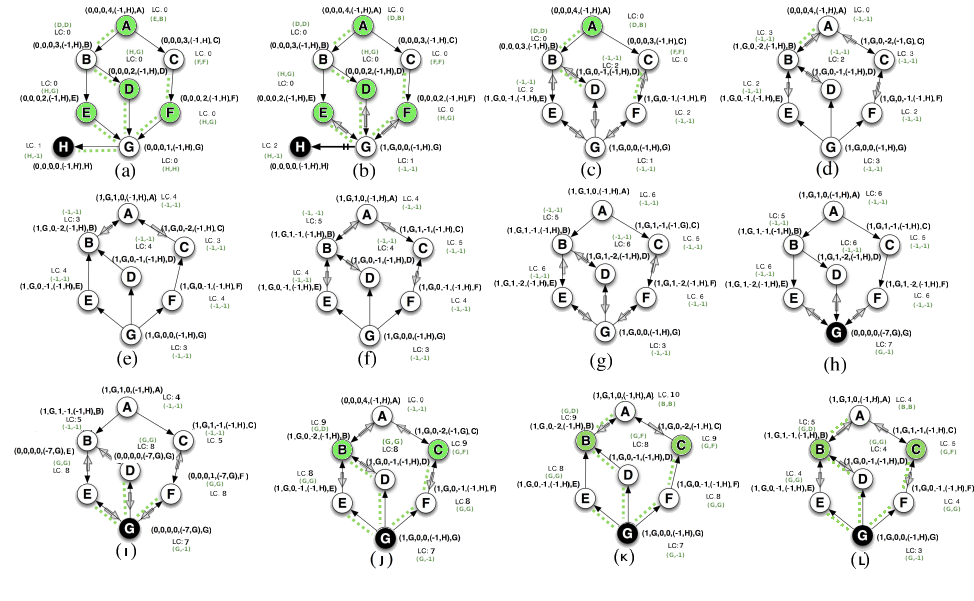
\includegraphics[width=1\linewidth]{test_1}
	\caption{Simple execution when leader H becomes disconnected (a), with time increasing from (a)–(l). With no other link changes, every node in the connected component will eventually adopt G as its leader and a new leaders' hierarchy will be established.}
	\label{fig:test1}
\end{figure}

\end{landscape}
\chapter{Correctness}
\paragraph{}In this section, we show that, once topology changes cease, the algorithm eventually terminates with each connected component being leader-oriented. As a result, the $lid_u$ variables satisfy the conditions of the leader election problem.
\paragraph{}We first show, in Section 4.1, an important relationship between the final communication topology and the forming and $N$ variables of the nodes. The rest of the proof uses a number of invariants, denoted as “Properties”, which are shown to hold in every configuration of every execution; each one is proved (separately) by induction on the configurations occurring in an execution. In Section 4.2, we introduce some definitions and basic facts regarding the information about nodes' heights that appears in the system, either in nodes' height arrays or in messages in transit. In Section 4.3, we bound, in Lemma 3, the number of elections that can occur after the last topology change; this result relies on the fact, shown in Lemma 2, that once a node $u$ adopts a leader that was elected after the last topology change, $u$ never becomes a sink again. Then in Section 4.4, we bound, in Lemma 4, the number of new reference levels that are started after the last topology change; the proof of this result relies on several additional properties. Section 4.5 is devoted to showing, in Lemmas 5, 6, and 7, that eventually there are no messages in transit and every node has an accurate view of its neighbors' heights. All the pieces are put together in Theorem 1 of Section 4.6 to show that eventually we have a leader-oriented connected component; a couple of additional properties are needed for this result.
\paragraph{}Throughout the proof, consider an arbitrary execution of the algorithm in which the last topology change event occurs at some global time $t_{LTC}$, and consider any connected component of the final topology.
\section{Channels and Neighbors}
\paragraph{}Because of the lack of coordination between the topology change events for the two channels going between nodes $u$ and $v$ in the two directions, $u$ and $v$ do not necessarily have consistent views of their local neighborhoods in $G_{chan}$, even after the last topology change. For instance, it is possible that $v$ is in $N_u$ but $u$ is not in $N_v$ forever after the last topology change. Suppose the channel from $u$ to $v$ remains $Up$ from some time $t$ onwards, so that $v$ remains in $N_u$ from time $t$ onwards. However, suppose that the channel from $v$ to $u$ fluctuates several times after time $t$, eventually stabilizing to being $Up$ (cf. Fig. 5). Every time the channel to $u$ goes down, $u$ is removed from $v$'s forming and $N$ sets. Every time the channel to $u$ comes up, $v$ adds $u$ to $forming_v$ and sends its height in an $Update$ message to $u$. When $u$ gets the message from $v$, it updates the entry for $v$ in its height array, but does not send its own height back to $v$. As long as $u$'s height does not change, $u$ does not send its height to $v$. Thus $v$ is never able to move $u$ from $forming_v$ into $N_v$.
\begin{figure}[h]
	\centering
	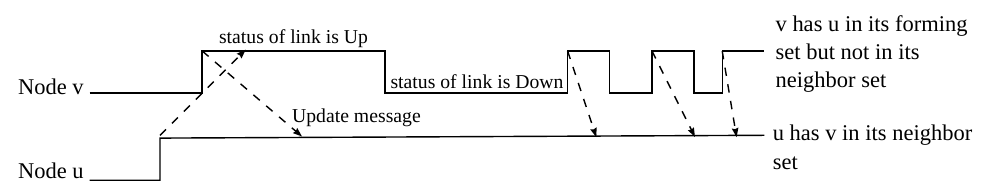
\includegraphics[width=1\linewidth]{fig_1}
	\caption[The status of the channel from $u$ to $v$ remains $Up$, but the status of the channel from $v$ to $u$ fluctuates.]{The status of the channel from $u$ to $v$ remains $Up$, but the status of the channel from $v$ to $u$ fluctuates.}
	\label{fig:fig1}
\end{figure}
\paragraph{}However, we are assured by Lemma 1 below that after time $t_{LTC}$ , $N_u \cup forming_u$ does not change for any node $u$. Furthermore, a node $u$ always sends $Update$ messages to all nodes in $N_u \cup forming_u$ , which constitutes all the outgoing channels of $u$.
\paragraph{Lemma 1}After time $t_{LTC}$, $N_u \cup forming_u$ does not change for any node $u$.
\subparagraph{Proof}When $ChannelDown_{uv}$ occurs, $u$ removes $v$ from both its $N_u$ and $forming_u$ variables. When $ChannelUp_{uv}$ occurs, $u$ adds $v$ to its $forming_u$ variable and sends an $Update$ message to $v$. When $u$ receives an $Update$ message from a node $v$, the only possible change to the $N_u$ and $forming_u$ variables is that $v$ is moved from $forming_u$ to $N_u$, which does not change $N_u \cup forming_u$.
\subparagraph{}$t_{TLC}$ is the latest among all the times at which either a $ChannelDown$, or a $ChannelUp$ occurs. After this time, the only change to the $N$ set or the forming set must be due to receipt of an $Update$ message, causing lines 2 and 3 of Figure 2 to be executed. Thus the only change to the $N$ set or the forming set is that a node which is removed from the forming set is added to the $N$ set. This does not affect $N \cup forming$.
\section{Height Tokens and Their Properties}
\paragraph{}Since a node makes algorithm decisions based solely on comparisons of its neighboring nodes' height tuples, we first present several important properties of the tuple contents. Define $h$ to be a height token for node $u$ in a configuration if $h$ is in an $Update$ message in transit from $u$, or $h$ is the entry for $u$ in the height array of any node. Let $LP(h)$ be the leader pair of $h$, $RL(h)$ the reference level (triple) of $h$, $\delta(h)$ the $\delta$ value of $h$, $lts(h)$ the absolute value of the (non-positive) leader timestamp (component $nlts$) of $h$, and $\tau (h)$ the $\tau$ value of $h$.
\paragraph{}Given a configuration in which $Channel(u, v)$ has status $Up$ and $u \in N_v$ , the $(u, v)$ height sequence is defined as the sequence of height tokens $h_0, h_1, ... , h_m$, where $h_0$ is $u$'s height, $h_m$ is $v$'s view of $u$'s height, and $h_1, ..., h_{m-1}$ is the sequence of height tokens in the $Update$ messages in transit from $u$ to $v$. If the status of $Channel(u, v)$ is $Up$ but $u \not\in N_v$ , then the $(u, v)$ height sequence is defined similarly except that $h_1, ... , h_m$ is the sequence of height tokens in the $Update$ messages in transit from $u$ to $v$; in these cases, $v$ does not have an entry for $u$ in its height array. If $Channel(u, v)$ is $Down$, the $(u, v)$ height sequence is undefined.
\paragraph{Property A}If $h$ is a height token for a node $u$ in the $(u, v)$ height sequence, then:
\begin{enumerate}
	\item $lts(h) \leq \mathcal{T} _u$ and $\tau (h) \leq \mathcal{T} _u$
	\item If $h$ is in $v$'s height array then $lts(h) \leq \mathcal{T} _v$ and $\tau (h) \leq \mathcal{T} _v$ .
\end{enumerate}
\newpage

\subparagraph{Proof}By induction on the configurations in the execution.
\subparagraph{}\textit{Basis:} In the initial configuration $C_0$ , all the leader timestamps and $\tau$ values are $0$ and $\mathcal{T} \geq 0$ for all nodes $v$.
\subparagraph{}\textit{Inductive Hypothesis:} Suppose the property is true in configuration $C_{i-1}$ and show it remains true in configuration $C_i$. Since the property is true in $C_{i-1}$ , for every height token $h$ in the $(u, v)$ height sequence, we have:
\begin{enumerate} [label=(\roman*)]
	\item $lts(h) \leq \mathcal{T} _u(C_{i-1})$ and $\tau (h) \leq \mathcal{T} _u(C_{i-1})$
	\item If $h$ is in $v's$ height array then $lts(h)$ $\leq$ $\mathcal{T} _v(C_{i-1})$ and $\tau (h)$ $\leq$ $\mathcal{T} _v (C_{i-1})$
\end{enumerate}
\subparagraph{}\textit{Inductive Step:} If $h$ is a preexisting height token during event $e_i$ (the event immediately preceding $C_i$), then by the inductive hypothesis and the increasing property of $\mathcal{T} _u$, it follows that $lts(h) \leq \mathcal{T} _u (C_i)$ and $\tau (h) \leq \mathcal{T} _u(C_i)$. If, on the other hand, $h$ is created during event $e_i$, then any new values of $lts$ and $\tau$ generated by $u$ are equal to $\mathcal{T} _u(C_i)$ and, thus, the property remains true.
\subparagraph{}If $h$ is a height token for node $u$ at some other node $v$, then $h$ was either present at $v$ during $C_{i-1}$ or was received at $v$ during event $e_i$, immediately preceding $C_i$. In the first case, by the inductive hypothesis and the increasing property of $\mathcal{T} _v$, it follows that $lts(h) \leq \mathcal{T} _v (C_i)$ and $\tau (h) \leq \mathcal{T} _v (C_i)$. In the second case, there exists a message through which $v$ received $h$ from $u$ during event $e_i$ . Since $\mathcal{T}$ preserves causality, by the definition of the happens before relation, it follows that the creation of either $\tau (h)$ or $lts(h)$ preceded the receipt of the message by $v$. Therefore, in configuration $C_i$ it remains true that $lts(h) \leq \mathcal{T} _v (C_i)$ and $\tau (h) \leq \mathcal{T} _v (C_i)$.
\paragraph{}Property B, given below, states some important facts about height sequences. If the channel's status is $Up$ and $m = 1$, meaning that no messages are in transit from $u$ to $v$, then Part (1) of Property B indicates that $v$ has an accurate view of $u$'s height. If there are $Update$ messages in transit, then the most recent one sent has accurate information. Part (2) of Property B implies that leader pairs are taken on in decreasing order. Part (3) of Property B implies that reference levels are taken on in increasing order with respect to the same leader pair. Note that Property B only holds if $m > 0$.
\paragraph{Property B:}Let $h_0, h_1, ... , h_m$ be the $(u, v)$ height sequence for any $Channel(u, v)$ whose status is $Up$. Then the following are true if $m > 0$:
\begin{enumerate}
	\item $h_0 = h_1$.
	\item For all $l$, $0 \leq l < m,~LP(h_l ) \leq LP(h_{l+1} )$.
	\item For all $l$, $0 \leq l < m,$ if $LP(h_l ) = LP(h_{l+1})$, then $RL(h_l) \geq RL(h_{l+1})$.
\end{enumerate}
\paragraph{Proof}The proof is by induction on the execution.
\subparagraph{}Initially in $C_0$, $Channel(u, v)$ is either $Up$ or $Down$. If $Channel(u, v)$ is $Down$, then the $(u, v)$ height sequence is undefined. If $Channel(u, v)$ is $Up$, then the definition of initial configurations states that no messages are in transit and $v$ has an accurate view of $u$'s height, that is, $m = 1$ and $h_0 = h_1$.
\subparagraph{}Suppose the property is true in configuration $C_{i-1}$ and show it is still true in configuration $C_i$.
\subparagraph{}Suppose event $e_i$ is $ChannelDown_{uv}$. Then the $(u, v)$ height sequence is not defined in $C_i$.
\subparagraph{}Suppose event $e_i$ is $ChannelUp_{uv}$. By the assumption that the channel up/down events for a given channel alternate, the state of the channel in $C_{i-1}$ is Down and there are no messages in transit. Thus in $C_i$ the $(u, v)$ height sequence is $h$, where $h$ is the height of $u$ in $C_i$, which is stored in $u's$ height array and is in the $Update$ message that $u$ sends to $v$. Clearly this height sequence satisfies the three conditions.
\subparagraph{}Suppose event $e_i$ is the receipt by $v$ of an $Update$ message from $u$. In one case, the $(u, v)$ height sequence changes by dropping the last element, if the oldest message in transit takes the place of $v's$ view of $u's$ height. In the other case, the $(u, v)$ height sequence does not change if the receipt causes $v$ to record $u's$ height and add $u$ to $N_v$. In both cases, the three conditions still hold.
\subparagraph{}Suppose event $e_i$ is the receipt by $u$ of an $Update$ message from node $w$ or is a $ChannelDown$ event for a channel to some node other than $v$. If $u$ does not change its height, then there is no change affecting the property.
\subparagraph{}Suppose $u$ changes its height from $h' _0$ to $h$.
\subparagraph{}Let the $(u, v)$ height sequence in $C_{i-1}$ be $h' _0 , h'_1, ... , h'_m$. By the inductive hypothesis, $h' _0 = h' _1$ . By the code, the $(u, v)$ height sequence in $C_i$ is $h, h, h'_1 , ... , h'_m$. In each case we just have to show that $h$ has the proper relationship to $h'_1$, which equals $h'_0$.
\subparagraph{}Case 1: $e_i$ calls $REFLECTREFLEVEL$: All of $u's$ neighbors are viewed as having the same $LP$ as $u$, having reference level $(t, p, 0)$ for some $t$ and $p$, and having a larger height than $u$.
\subparagraph{}Since $u$ is a sink during the step, $RL(h'_0 )$ $\leq$ $(t, p, 0)$. Since $RL(h) = (t, p, 1)$, and the old and new $LP$ are the same, the property holds.
\subparagraph{}Case 2: $e_i$ calls $ELECTSELF$: By Property A, $lts$ in $LP(h'_0 )$ is less than or equal to $\mathcal{T} _{u'}$ in configuration $C_{i-1}$. The new leader pair has $lts~\mathcal{T} _u$ in configuration $C_i$, which is greater than $\mathcal{T} _{u'}$. So $LP(h)$ $\leq$ $LP(h'_0 )$.
\subparagraph{}Case 3: $e_i$ calls $STARTNEWREFLEVEL$: By Property A, the $\tau$ value in $RL(h'_0 )$ is less than or equal to $\mathcal{T}_u'$ at configuration $C_{i-1}$. The new reference level has $\tau$ value $\mathcal{T}_u$ at configuration $C_i$, which is greater than $\mathcal{T}_{u'}$ and the $LP$ is unchanged. So $LP(h) = LP(h'_0 )$ and $RL(h)$ $\geq$ $RL(h'_0 )$.
\subparagraph{}Case 4: $e_i$ calls $PROPAGATELARGESTREFLEVEL$: All neighbors of $u$ are viewed as having the same $LP$ as $u$, but with different $RLs$ among themselves, and as having larger heights than $u$. By the code, $u$ takes on the largest neighboring $RL$, which is at least as large as $u's$ old $RL$, since $u$ is a sink. The $LP$ is unchanged. So $LP(h) = LP(h'_0 )$ and $RL(h)$ $\geq$ $RL(h'_0 )$.
\subparagraph{}Case 5: $e_i$ calls $ADOPTLPIFPRIORITY$: By the code, the new $LP$ is smaller than the previous, so $LP(h) < LP(h'_0 )$.
\newpage
\section{Bounding the Number of Elections}
\paragraph{}In this subsection, we show that every node elects itself at most a finite number of times after the last topology change.
\paragraph{}Define the following with respect to any configuration in the execution. For $LP (-s, l)$, where $\mathcal{T}_l (t) = s$ and $t$ $\geq$ $t_{LTC}$, let $LP$ tree $LT (-s, l)$ be the sub-graph of the connected component whose vertices consist of all nodes that have taken on $LP (-s, l)$ in the execution (even if they no longer have that $LP$), and whose directed edges are all ordered pairs $(u, v)$ such that $v$ adopts $LP (-s, l)$ due to the receipt of an $Update$ message from $u$. Since a node can take on a particular $LP$ only once by Property B, $LT (-s, l)$ is a tree rooted at $l$.
\paragraph{Porperty C:}For each height token $h$ with $RL (t, p, r)$, either $t = p = r = 0$, or $t > 0$, $p$ is a node $id$, and $r$ is $0$ or $1$.
\subparagraph{Proof}The proof is by induction on the sequence of configurations in the execution. The basis follows since all height tokens in an initial configuration have $RL (0, 0, 0)$.
\subparagraph{}For the inductive step, we consider all the ways that a new $RL$ can be generated (as opposed to copying an existing one). In $ELECTSELF$, the new $RL$ is $(0,0,0)$. In $STARTNEWREFLEVEL$ , the new RL is $(t, p, 0)$, where $t$ is the current causal clock time, which is positive, and $p$ is a node $id$. In $REFLECTREFLEVEL$, the new $RL$ is $(t, p, 1)$, where $(t, p, 0)$ is a preexisting height token. By the precondition for executing $REFLECTREFLEVEL$, $t$ is positive. By the inductive hypothesis applied to the preexisting height token $(t, p, 0)$, $p$ is a node $id$.
\paragraph{Property D:}Let $h$ be a height token for some node $u$. If $LP(h) = (-s, l)$, where for some global time $t$, $T_l (t) = s$ and $t \geq t_{LTC}$ , then $RL(h) = (0, 0, 0)$ and $\delta (h)$ is the distance in $LT (-s, l)$ from $l$ to $u$.
\subparagraph{Proof:}By induction on the sequence of configurations in the execution.
\subparagraph{}By Property A, the basis is configuration $C_j$, just after the event at global time $t$ when the first height tokens with $LP (-s, l)$ are created. By the code, these height tokens are created by node $l$ for itself and have $RL (0, 0, 0)$ and $\delta = 0$.
\subparagraph{}Assume the property is true in configuration $C_{i-1}$ , with $i-1$ $\geq$ $j$, and show it is true in configuration $C_i$. Since no further topology changes occur, the only possibility for event $e_i$ is the receipt of an $Update$ message. Suppose node $u$ receives $Update(h)$ from node $v$.
\subparagraph{}As a result of the receipt of the message, $u$ records $h$ as $v$'s height in its view. The inductive hypothesis implies that the property remains true for this new height token.
\subparagraph{}Also as a result of the receipt of the message, $u$ might change its height.
\subparagraph{}Suppose $u$ changes its height by executing $ADOPTLPIFPRIORITY$, adopting the $LP$ in $h$, where $LP(h) = (-s, l)$. By the inductive hypothesis, $RL(h) = (0, 0, 0)$, and $\delta (h)$ is the distance from $l$ to $v$ in $LT (-s, l)$ in $C_{i-1}$. By Property B, since $u$ adopts $(-s, l)$, it must be that $u's$ $LP$ is larger than $(-s, l)$ in $C_{i-1}$ , and thus $v$ is $u's$ parent in $LT (-s, l)$. By the code, $u$ sets its $RL$ to $(0, 0, 0)$ and its $\delta$ to $\delta (h) + 1$. But this is exactly the distance in $LT (-s, l)$ from $l$ to $u$. So all height tokens created in this step satisfy the property.
\subparagraph{}Suppose $u$ changes its height because it becomes a sink and $u's$ new height has $LP (-s, l)$. First, we show that $u$ does not take on $LP (-s, l)$ as a result of $ELECTSELF$. By assumption, $LP (-s, l)$ is created in configuration $C_j$ (the base case). By the code and the increasing property of causal clocks, it follows that $l$ cannot create a duplicate of $LP (-s, l)$ at some later configuration $C_i$. Therefore, $u$ does not take on $LP (-s, l)$ as a result of $ELECTSELF$.
\subparagraph{}Thus, the old height of $u$, call it $h'$, also has $LP (-s, l)$. Since $u$ becomes a sink, all its neighbors have $LP (-s, l)$ in $u's$ view, and by the inductive hypothesis they all have $RL (0, 0, 0)$ in $u's$ view. Thus the new height of $u$ is not the result of executing $REFLECTREFLEVEL$ (which requires the neighbors' common $\tau$ to be positive) or $PROPAGATELARGESTREFLEVEL$ (which requires the neighbors to have different $RL's$). Instead, it must be the result of executing $STARTNEWREFLEVEL$. Since $u$ is a sink and $(0, 0, 0)$ is the smallest possible $RL$ by Property C, $RL(h' ) = (0, 0, 0)$. Also, since $u$ is a sink, $u = l$. Let $v$ be $u's$ parent in the $LP-tree~LT (-s, l)$ and let $d$ be the distance in that tree from $l$ to $v$. By the inductive hypothesis, in $u's$ view of $v's$ height, $v's$ $\delta = d$, but in $u's$ own height, $\delta = d + 1$. Thus the edge between $u$ and $v$ is directed toward $v$, and $u$ cannot be a sink, a contradiction.
\paragraph{Lemma 2}Any node $u$ that adopts leader pair $(-s, l)$ for any $l$ and any $s$, where for some global time $t$, $\mathcal{T}_l (t) = s$ and $t > t_{LTC}$ , never subsequently becomes a sink.
\subparagraph{Proof}Suppose in contradiction that $u$ adopts leader pair $(-s, l)$ at global time $t_1 > t$ and that at global time $t_2 > t_1$, $u$ becomes a sink. Suppose $u$ does not change its leader pair in the time interval $(t_1 ,t_2 )$. (If $u$ did change its leader pair, the new leader pairs would all be smaller than $(-s, l)$ by Property B, and the argument would still hold with respect to the latest leader pair taken on by $u$ in that time interval.)
\subparagraph{}Let $v$ be the parent of $u$ in the $LP$-tree $LT(-s, l)$. Immediately after time $t_1$, the link $(u, v)$ is directed from $u$ to $v$ in $u's$ view.
\subparagraph{}In order for $u$ to become a sink at time $t_2$ , there must be some time between $t_1$ and $t_2$ when the link $(u, v)$ reverses direction in $u's$ view. Suppose the link reverses because $u's$ height lowers. Recall that $u$ does not change its leader pair in $(t_1,t_2 )$ by assumption. By Property D, $u's$ reference level remains $(0, 0, 0)$ in $(t_1 ,t_2 )$ and $u's$ $\delta$ stays the same in the interval. That is, $u's$ height does not change, and in particular does not lower. Thus the only way that the link $(u, v)$ can reverse direction in $(t_1 ,t_2 )$ is due to the receipt by $u$ of an update message from $v$ with a new height for $v$ that is higher than $u's$ height.
\subparagraph{}How can $v's$ height change after $v$ takes on leader pair $(-s, l)$ ? One possibility is that $v's$ leader pair changes. By Property B, any change in $v's$ leader pair will be to a smaller one, which will be adopted by $u$ together with a $\delta$ value that keeps the link directed from $u$ to $v$ in $u's$ view.
\subparagraph{}The other possibility is that $v$'s leader pair does not change but some other component of its height changes. But by Property D, since $v$'s leader pair has timestamp $-s$ with $\mathcal{T} _l (t) = s$ and $t > t_{LTC}$ , $v$'s RL and $\delta$ cannot change.
\subparagraph{}Thus no change to $v's$ height reported to $u$ after time $t_1$ can cause the link $(u, v)$ to be directed from $v$ to $u$ in $u's$ view, and $u$ cannot be a sink at time $t_2$ , which is a contradiction.
\paragraph{Lemma 3}No node elects itself more than a finite number of times after global time $t_{LTC}$.
\subparagraph{Proof}Suppose in contradiction that a node $u$ elects itself an infinite number of times after the last topology change. Once it has elected itself the first time, the only way it can become a sink and elect itself again is by adopting a new $LP$ first. Thus, node $u$ needs to adopt new $LP's$ infinitely often after $t_{LTC}$ . By Property B, the leader timestamp of each subsequent $LP$ has to be greater than the previous one, which results in an increasing sequence of leader timestamps that $u$ adopts. Let $\mathcal{T}_{max}$ be the maximum of the clocks of all nodes at time $t_{LTC}$. In the process of adopting increasing leader timestamps, at some point $u$ will adopt $LP(-s, l)$ where $\mathcal{T} _l (t) = s$ and for which $s > \mathcal{T} _{max}$.
\subparagraph{}This follows from the first property of causal clocks which states that for each node $u$, the values of $\mathcal{T}_u$ are increasing, i.e., if $e_i$ and $e_j$ are events involving $u$ in the execution with $i < j$, then $\mathcal{T} _u (e_i ) < \mathcal{T} _u (e_j )$, and, furthermore, if there is an infinite number of events involving $u$, then $\mathcal{T} _u$ increases without bound. 
\subparagraph{}Because $\mathcal{T} _{max}$ was the maximum value of all clocks at the time of the last topology change, it follows that $t > t_{LTC}$. By Lemma 2, however, node $u$ does not become a sink after it has adopted $LP(-s, l)$ and thus it cannot elect itself again after that time, which is a contradiction.
\subparagraph{}If we use perfect clocks to implement $\mathcal{T}$ , we can get a stronger bound on the number of times a node elects itself after the last topology change. In fact, with perfect clocks it is guaranteed that no node elects itself more than once after the last topology change, as we now explain. As stated in the proof of Lemma 3, if a node $u$ elects itself more than once after the last topology change, it must take on a new $LP$ in between each successive pair of elections. Also, by Property B, the timestamps in these $LP's$ must be increasing. As explained in the proof of Lemma 3, there could be multiple $LPs$ already existing at the time of the last topology change whose timestamps are greater than the timestamp of the $LP$ that $u$ takes on the first time it elects itself after the last topology change. The reason is that the clocks are causal, yet are drawn from a totally-ordered set, and thus just because clock value $t_1$ is less than clock value $t_2$ , it does not follow that the event associated with $t_1$ happened before the event associated with clock value $t_2$. However, the number of such misleading timestamps is finite, so eventually, if $u$ keeps electing itself, it will take on a timestamp that is associated with an event that occurred after the last topology change. Then we can apply Lemma 2 to deduce that $u$ will never elect itself again. When clocks are perfect, however, there can be no such misleading timestamps in $LP's$: if the timestamp in a new $LP$ is greater than the timestamp taken on by $u$ the first time, then this $LP$ was definitely generated after the last topology change and Lemma 2 applies immediately. For more details, refer to Lemma 3 in [15].
\section{Bounding the Number of New Reference Levels}
\paragraph{}In this subsection, we show that every node starts a new reference level at most a finite number of times after the last topology change. The key is to show that after topology changes cease, nodes will not continue executing Line 13 of Figure 2 infinitely and will therefore stop sending algorithm messages. First we show that the $\delta$ value of a node does not change unless its $RL$ or $LP$ changes.
\paragraph{Property E:}If $h$ and $h'$ are two height tokens for the same node $u$ with $RL(h) = RL(h')$ and $LP(h) = LP(h')$, then $\delta (h) = \delta (h' )$.
\subparagraph{Proof}Initially, in $C_0$, the only height tokens for node $u$ are the ones in $u$ and the ones in $u's$ neighbors, and the neighbors have accurate views of $u's$ height.
\subparagraph{}Suppose the property is true through configuration $C_{i-1}$. We will show it is still true in the next configuration $C_i$. The only way that new height tokens can be introduced into the system is if a node $u$ changes its height and sends $Update$ messages with the new height to its neighbors.
\subparagraph{}Suppose $u$ changes its height through $ELECTSELF$ (resp., $STARTNEWREFLEVEL$). Since the new height's leader timestamp (resp., $\tau$ ) is the value of the logical clock of $u$, Property A implies that there is no preexisting height token for $u$ in the system with the new leader timestamp (resp., $\tau$ ). Thus there cannot be two height tokens for $u$ with the same $RL$ and $LP$ but conflicting $\delta s$ .
\subparagraph{}Suppose $u$ changes its height through $ADOPTLPIFPRIORITY$. Then the new height of $u$ has a smaller $LP$ than the old height. By Property B, there is no preexisting height token for $u$ in the system with the new LP. Thus there cannot be two height tokens for $u$ with the same $RL$ and $LP$ but conflicting $\delta s$.
\subparagraph{}Suppose $u$ changes its height through $REFLECTREFLEVEL$. Since $u$ is a sink and in its view all its neighbors have a common, unreflected, $RL$, call it $(t, p, 0)$, $u's$ $RL$ must be at most $(t, p, 0)$. Since $u's$ new RL is $(t, p, 1)$, Property B implies that there is no preexisting height token for $u$ in the system with the new RL. Thus there cannot be two height tokens for $u$ with the same $RL$ and $LP$ but conflicting $\delta s$ . 
\subparagraph{}Suppose $u$ changes its height through $PROPAGATELARGESTREFLEVEL$. The precondition includes the requirement that not all the neighbors have the same $RL$ (in $u's$ view). Since $u$ becomes a sink, $u's$ old RL is less than the largest $RL$ of its neighbors, which is the $RL$ that $u$ takes on in $C_i$. Property B implies that there is no preexisting height token for $u$ in the system with the new $RL$. 
\subparagraph{}Thus there cannot be two height tokens for $u$ with the same $RL$ and $LP$ but conflicting $\delta s$.

\paragraph{}The next definition and its related properties are key to understanding how unreflected and reflected reference levels spread throughout the connected component after the last topology change.
\paragraph{}Define the following with respect to any configuration in the execution after $t_{LTC}$. For global time $t'$ $\geq$ $t_{LTC}$, let the $RL$ DAG $RL (t, u, 1)$, where $REFLECTREFLEVEL$. Since $u$ is a sink and in its view all its neighbors have a common, unreflected, $RL$, call it $(t, p, 0)$, $u's$ $RL$ must be at most $(t, p, 0)$. Since $u's$ new RL is $(t, p, 1)$, Property B implies that there is no preexisting height token for $u$ in the system with the new $RL$. Thus there cannot be two height tokens for $u$ with the same $RL$ and $LP$ but conflicting $\delta s$ . 
\subparagraph{}Suppose $u$ changes its height through $PROPAGATELARGESTREFLEVEL$. The precondition includes the requirement that not all the neighbors have the same $RL$ (in $u's$ view). Since $u$ becomes a sink, $u's$ old $RL$ is less than the largest $RL$ of its neighbors, which is the $RL$ that $u$ takes on in $C_i$. Property B implies that there is no preexisting height token for $u$ in the system with the new $RL$. 
\subparagraph{}Thus there cannot be two height tokens for $u$ with the same $RL$ and $LP$ but conflicting $\delta s$.

\paragraph{}The next definition and its related properties are key to understanding how un-reflected and reflected reference levels spread throughout the connected component after the last topology change.
\paragraph{}Define the following with respect to any configuration in the execution after $t_{LTC}$. For global time $t'$ $\geq$ $t_{LTC}$, let the $RL$ DAG $RL (t, u, 1)$, where $\mathcal{T}_p(t ' ) = t$, be the sub-graph of the connected component whose vertices consist of $p$ and all nodes that have taken on $RL$ prefix $(t, p)$ by executing either $PROPAGATELARGESTREFLEVEL$ or $REFLECTREFLEVEL$ in the execution (even if they no longer have that RL prefix). In $RL (t, u, 1)$, the directed edges are all ordered pairs of node ids $(u, v)$ such that $u$ $\in$ $N_v$ and $v$ $\in$ $N_u$ and $u$ has $RL$ prefix $(t, p)$ prior to the event in which $v$ first takes on $RL$ prefix $(t, p)$. We say that node $u$ is a predecessor of node $v$ in $RL (t, u, 1)$ and $v$ is a successor of $u$ in $RL (t, u, 1)$.

\paragraph{Property F:} If there is a height token for node $u$ with $RL$ prefix $(t, p)$, where $\mathcal{T}_p(t') = t$ and $t'$ $\geq$ $t_{LTC}$ , then $u$ is in $RL (t, u, 1)$.
\subparagraph{Proof} By induction on the sequence of configurations in the execution.
\subparagraph{}The basis is configuration $C_j$, where $gt(C_j ) = t '$ , i.e., the time when node $p$ starts $RL (t, p, 0)$. By Property A, there is no height token with $RL$ prefix $(t, p)$ in $C_{j-1}$ , so the only height tokens we have to consider are those created by $p$, for $p$. By definition, $p$ is in $RL (t, u, 1)$.
\subparagraph{}Suppose the property is true through configuration $C_{i-1}$. We will show it is true in $C_i$.
\subparagraph{}Suppose in contradiction, in event $e_i$, some node $u$ takes on $RL$ prefix $(t, p)$ by calling $ADOPTLPIFPRIORITY$ after receiving an update message from neighbor $v$ containing height $h$ with $RL$ prefix $(t, p)$. By the inductive hypothesis, $v$ is in $RL (t, u, 1)$.
\subparagraph{}Let $(-s, l)$ be $LP(h)$. We are going to show that when $v$ takes on $RL$ prefix $(t, p)$, final it already has $LP (-s, l)$. We know that $v$ must have a path to node $p$ in $G_{chan} ^{final}$ that has been in place since $p$ started the new $RL$ prefix at time $t$, by the assumption that topology changes have stopped by real time $t'$. Just before time $t'$, all the neighbors of $p$ had $LP (-s, l)$ and $RL$ prefix lower than $(t, p)$, by Property B, or $p$ would not have started a new reference level for $LP (-s, l)$. Since the neighbors of $p$ had $LP (-s, l)$, they would have sent messages containing that $LP$ to their neighbors prior to time $t'$. Likewise, those neighbors would have messages in transit to their neighbors containing the $LP (-s, l)$ and so on. In short, if the $LP (-s, l)$ is adopted by any nodes that have a path to $p$ at $t'$, then the $LP$ would have been adopted when that $LP$ spread through the network with a lower $RL$ prefix. 
\subparagraph{}Thus, when $v$ puts $h$ in transit to $u$, there is already ahead of it in the $(v, u)$ height sequence a height token for $v's$ old height, with $LP (-s, l)$. Since the channels are FIFO and no messages are lost after time $t'$, $u$ has already received the old height from $v$ before $e_i$. So in $C_{i-1}$, $u$ has a $LP$ that is $(-s, l)$ or smaller already, before handling the Update message with height $h$. Thus $u$ does not execute $ADOPTLPIFPRIORITY$ in $e_i$, contradiction.
\paragraph{Property G:} If there is a height token for node $u$ with $RL (t, p, 1)$, where for some global time $t '$, $\mathcal{T}_p(t') = t$ and $t '$ $\geq$ $t_{LTC}$, then all neighbors of $u$ are in $RL (t, u, 1)$.
\subparagraph{Proof} By induction on the sequence of configurations in the execution.
\subparagraph{}The basis is the configuration $C_j$ with $gt(C_j ) = t '$, i.e., the time when the new $RL$ is started at node $p$. By Property A, there is no height token in $C_{j-1}$ with $RL (t, p, 1)$, and in $C_j$ we only add height tokens for node $p$ with $RL (t, p, 0)$. So the property is vacuously true.
\subparagraph{}Suppose the property is true through configuration $C_{i-1}$ and show it is true in $C_i$, $i > j$.
\subparagraph{}By Property F and the definition of $RL (t, u, 1)$, the only way that $u$ can take on $RL (t, p, 1)$ is by $REFLECTREFLEVEL$ or $PROPAGATELARGESTREFLEVEL$.
\subparagraph{}Suppose $u$ takes on $RL (t, p, 1)$ due to $REFLECTREFLEVEL$. Then all $u's$ neighbors have $RL (t, p, 0)$ in its view. By Property F, then, they are all in $RL (t, u, 1)$.
\subparagraph{}Suppose $u$ takes on $RL (t, p, 1)$ due to $PROPAGATELARGESTREFLEVEL$. Thus there is a height token in $C_{i-1}$ for some neighbor $v$ of $u$ with $RL (t, p, 1)$. By the inductive hypothesis applied to $v$, all of $v's$ neighbors, including $u$, are in $RL (t, u, 1)$. Thus $u's$ $RL$ prefix at some earlier time is $(t, p)$. By Property B (since the $LP$ does not change in this interval), $u's$ $RL$ prefix in $C_{i-1}$ is at least $(t, p)$. Since $u$ is a sink during event $e_i$, $u's$ $RL$ prefix in $C_{i-1}$ is at most $(t, p)$, so it is exactly $(t, p)$ in $C_{i-1}$. Since $u$ is a sink, every neighbor of $u$ (in $u's$ view) has $RL$ prefix at least $(t, p)$, and since $(t, p, 1)$ is the maximum of the neighboring $RL's$, every neighbor of $u$ (in $u's$ view) has $RL$ prefix exactly $(t, p)$. Thus by Property F, every neighbor of $u$ is in $RL (t, u, 1)$.
\paragraph{Property H:} Suppose that $u$ and $v$ are two nodes such that $u$ $\in$ $N_v$ and $v$ $\in$ $N_u$ after $t_{LTC}$. Consider two height tokens, $h_u$ for node $u$ with $RL(h_u ) = (t, p, r_u )$ and $\delta (h_u )$ = $d_u$ , and $h_v$ for node $v$ with $RL(h_v ) = (t, p, r_v )$ and $\delta (h_v ) = d_v$, where $\mathcal{T}_p(t') = t$ and $t '$ $\geq$ $t_{LTC}$. Then the following are true: 
\begin{enumerate}
	\item If $r_u < r_v$ , then $u$ is a predecessor of $v$ in $RL (t, u, 1)$. If $u$ is a predecessor of $v$ in $RL (t, u, 1)$ then $r_u$ $\leq$ $r_v$.
	\item If $r_u = r_v = 0$, then $d_u > d_v$ if and only if $u$ is a predecessor of $v$.
	\item If $r_u = r_v = 1$, then $d_v > d_u$ if and only if $u$ is a predecessor of $v$.
\end{enumerate}
\subparagraph{Proof} By induction on the sequence of configurations in the execution. 
\subparagraph{}Basis: Consider configuration $C_j$, where $gt(C_j ) = t '$, that is, when node $p$ starts the new reference level $(t, p, 0)$. By Property A, in configuration $C_{j-1}$, there are no height tokens with $RL$ prefix $(t, p)$. The only new height tokens introduced by event $e_j$ are those for $p$ with $RL (t, p, 0)$, and the $RL$ DAG $RL (t, u, 1)$ consists solely of node $p$. Thus all parts of the property are vacuously true.
\subparagraph{}Induction: Assume the property holds through configuration $C_{i-1}$ and show it is true in $C_i$, $i > j$.
\subparagraph{}By Property E, it is sufficient to consider the height tokens in $u's$ view, since there cannot be other height tokens with the same $RL$ and $LP$ but different $\delta s$.
\subparagraph{}Suppose new height tokens with $RL$ prefix $(t, p)$ are created by node $u$ during event $e_i$. The only ways this can happen are via $REFLECTREFLEVEL$ and $PROPAGATELARGESTREFLEVEL$, by Property F.
\subparagraph{}CASE 1: $REFLECTREFLEVEL$. During the execution of $e_i$, all of $u's$ neighbors are viewed by $u$ as having $RL (t, p, 0)$ and the new height tokens created for $u$ have $RL (t, p, 1)$.
\subparagraph{}We now show that $u's$ $RL$ prefix is less than $(t, p)$ in $C_{i-1}$. Suppose in contradiction $u$ has $RL (t, p, 0)$ in $C_{i-1}$. By the inductive hypothesis, part (2), $u's$ $\delta$ value cannot be the same as that of any of its neighbors. This is true since $u$ and all its neighbors are in $RL (t, u, 1)$ by Property F, and, for any pair of neighboring nodes in $RL (t, u, 1)$, one is the predecessor of the other, since two events cannot happen simultaneously. Since $u$ is a sink, its $\delta$ value must be smaller than those of all its neighbors. By the inductive hypothesis, part (2), $u$ is a successor of all its neighbors, of which there is at least one.
\subparagraph{}Then at some previous time $t'' < gt(C_{i-1})$, $u$ executed $PROPAGATELARGES$-$TREFLEVEL$ and took on $RL (t, p, 0)$. This must be how $u$ took on $(t, p, 0)$ since, by Property F, $u$ cannot take on $RL (t, p, 0)$ by running $ADOPTLPIFPRIORITY$, and, if $u = p$, $u$ has no predecessors in $RL (t, u, 1)$, contradicting the deduction that $u$ is a successor of at least one neighbor. At $t''$, $u$ has (in its view) at least one neighbor with $RL (t, p, 0)$, $(t, p, 0)$ is the maximum $RL$ of all $u's$ neighbors, and at least one neighbor, say $v$, has a smaller $RL$ than $(t, p, 0)$, albeit larger than $u's$ (since $u$ is a sink).
\subparagraph{}Suppose $u$ has height $h_u$ at time $t''$, and its view of $v's$ height is $h_v$ at time $t''$. Since $u$ is a sink, $h_u$ and $h_v$ have the same leader pair, say $l_{p1}$, we have :
\begin{equation}
RL(h_u ) < RL(h_v ) < (t, p, 0)
\end{equation}
This means that there was a previous time $t ''' < t ''$ when $v$ actually took on height $h_v$ (with leader pair $lp_1$ ). We also know that $v$ has taken on $(t, p, 0)$ before time $t ''$, since $u$ is a successor of all its neighbors and it takes on $RL (t, p, 0)$ at time $t ''$ . Note that $v$ could not have taken on $RL (t, p, 0)$, with leader pair $lp_1$ before $t '''$. This is because at $t '''$ its leader pair is also $lp_1$ and its height $RL(h_v ) < (t, p, 0)$. By Property B two height tokens with the same leader pair must have increasing reference levels. Hence, $v$ took on $(t, p, 0)$ after $t '''$ and before $t ''$. Suppose $v$ took on $(t, p, 0)$ at time $s$ such that $t ''' < s < t ''$. We know that $v$ has to be a sink at time $s$ in order to do so. Thus at time $s$ all $v's$ neighbors in $v's$ view have the same leader pair as itself, and $v$ takes on $(t, p, 0)$ with leader pair $lp_1$ either by $PROPAGATELARGESTREFLEVEL$ or $STARTNEWREFLEVEL$. Suppose $v's$ own height is $h'_v$ at time $s$ and its view of $u's$ height is $h'_u$. Both $h'_v$ and $h'_u$ have leader pair $lp_1$ and, since $v$ is a sink we have
\begin{equation}
h'_v < h'_u
\end{equation}
Note that $h_v$, $h_u$, $h'_v$, and $h'_u$ all have leader pair $lp_1$. We also know that $h_u < h_v$ from (1). Now from Property B
\begin{equation}
h_v \leq h'_v
\end{equation}
Also from Property B
\begin{equation}
h_v \leq h'_v
\end{equation}
Hence, from (1), (3) and (4), we have
\begin{equation}
h'_u \leq h_u < h_v \leq h'_v
\end{equation}
\subparagraph{}This is in contradiction to (2).
\subparagraph{}Part (1): All neighbors of $u$ are its predecessors in $RL (t, u, 1)$ and in $C_i$, the predecessors of $u$ have $r = 0$ and $u$ has $r = 1$ so this part continues to hold.
\subparagraph{}Part (2): The creation of the new height tokens does not affect this part, since the new tokens do not have $r = 0$.
\subparagraph{}Part (3): Since $u$ is not in $RL (t, u, 1)$ in $C_{i-1}$ , Property G implies that there cannot be a height token for any of $u$'s neighbors with $RL (t, p, 1)$, and this part is vacuously true.
\subparagraph{}CASE 2: $PROPAGATELARGESTREFLEVEL$. In this case, $u's$ neighbors have at least two different $RL$s so we need to consider which $RL$ $u$ propagates, $(t, p, 0)$ or $(t, p, 1)$.

Case 2.1: Suppose $u$'s new height has $RL (t, p, 0)$. We first show that $u$ has $RL$ less than $(t, p, 0)$ in $C_{i-1}$. By the precondition for $PROPAGATELARGESTREFLEVEL$, in $u$'s view, $(t, p, 0)$ is the largest neighboring $RL$, at least one neighbor has $RL$ less than $(t, p, 0)$, and $u$ is a sink. Thus $u's~RL$ must be less than $(t, p, 0)$.

Part (1): Since the new height tokens of both $u$ and its predecessors have reflection bit $0$, this part is not invalidated in $C_i$.

Part (2): Each of $u's$ neighbors for which $u$ has a height token $h'$ with $RL (t, p, 0)$ is a predecessor of $u$ in $RL (t, u, 1)$, since $u$ is not yet in $RL (t, u, 1)$. By the code, $u's$ new height $h$ has a $\delta$ calculated so that $h' > h$.

Part (3): The new height tokens do not have reflection bit $1$ so this part is unaffected.

Case 2.2: Suppose $u$'s new height has $RL (t, p, 1)$. Then the largest $RL$ among $u's$ neighbors has, in u's view, $RL (t, p, 1)$. Property G implies that $u$ is in $RL (t, u, 1)$. So the $RL$ prefix of $u$ is at least $(t, p)$. Since $u$ is a sink, its $RL$ prefix is $(t, p)$ in $C_{i-1}$. So all neighbors (in $u's$ view) have $RL (t, p, 0)$ or $(t, p, 1)$ and there is at least one neighbor with each $RL$. Consider any neighbor $v$ of $u$ with $RL (t, p, 1)$ in $u$'s view. By the inductive hypothesis, part (1), $v$ must be a successor of $u$ in $C_{i-1}$.

Consider any neighbor $w$ of $u$ with $RL (t, p, 0)$ in $u's$ view. By the inductive hypothesis, part (2), $w$ must be a predecessor of $u$ in $C_{i-1}$ .

Part (1): Since $u$'s new height causes it to have the same reflection bit as its successors, and a larger reflection bit than its predecessors, this part continues to hold in $C_i$.

Part (2): Since the new height tokens do not have reflection bit $0$, this part is not affected.

Part (3): As argued above, each of $u$'s neighbors $v$ for which $u$ has a height token $h'$ with $RL (t, p, 1)$ is a successor of $u$ in $RL (t, u, 1)$. By the code, $u$'s new height $h$ has a $\delta$ calculated so that $h' > h$.
\paragraph{Lemma 4} Every node starts a finite number of new $RL$s after $t_{LTC}$.

\subparagraph{Proof} Suppose in contradiction that some node $u$ starts an infinite number of new $RL$s after $t_{LTC}$.

Now we show that $u$ takes on a new $LP$ infinitely often. Suppose in contradiction that $u$ does not do so. Let $t_{LLP}$ be the latest time at which $u$ takes on a new $LP$. Consider the first and second times that $u$ starts a new $RL$ (for the same $LP$) after $max\left\lbrace t_{LTC}, t_{LLP} \right\rbrace $; call these times $t_1$ and $t_2$.

At global time $t_1$ , $u$ sets its $\tau$ to $\tau _1$ . Since $u$ does not take on any more $LPs$, Property B implies that at the beginning of the step at time $t_2$, $u’s$ $\tau$ is at least $\tau _1$ , which is positive.

At the beginning of the event at time $t_2$, let $(t, p, r)$ be $u’s$ $RL$ and let $(t_c, p_c, r_c)$ be the common $RL$ of all $u’s$ neighbors (in $u’s$ view). Thus the precondition for starting a new $RL$ cannot be that $t_c = 0$, otherwise $u$ would not be a sink. So it must be that $t_c > 0$, $r_c = 1$, and $p_c \neq u$.

There are two cases, depending on the relationship between $(t, p)$ and $(t_c , p_c )$ (note that $(t, p)$ cannot be larger than $(t_c , p_c )$ since $u$ is a sink).

Case 1: $(t, p) < (t_c , p_c )$. Since $u$ has a height token with $RL (t_c , p_c , 1)$ for each neighbor $v$, we can apply Property G to deduce that all neighbors of $v$, including $u$, are in $RD(t_c , p_c )$. Thus, at some previous time, $u$ has $RL$ prefix $(t_c , p_c )$. But Property B implies that it is not possible for $u$ to have $RL$ prefix $(t_c , p_c )$ and then later to have $RL$ prefix $(t, p)$, since $(t, p) < (t_c , p_c )$.

Case 2: $(t, p) = (t_c , p_c )$. By Property F, node $u$ is in $RL (t, u, 1)$. Thus $u$ has a neighbor $v$ that is a predecessor of $u$ in $RL (t, u, 1)$.

Here we know that $v$ is in $N_u$. Also, since $v$ is a predecessor of $u$ in $RL (t, u, 1)$ $u$ is in $N_v$. Hence, we can apply Property H.

Since in $u’s$ view, $v$ has $RL (t, p, 1)$, Property H, Part (1), implies that $u’s$ reflection bit must also be $1$, and Property H, Part (3), implies that $u’s$ height must be greater than $v’s$. But this contradicts $u$ being a sink.

Since $u$ takes on a new $LP$ infinitely often, by Property B, the $lts$ values of the $LP’s$ that $u$ adopts are increasing without bound. Let $\mathcal{T} _{max}$ be the maximum of the clocks of all nodes at time $t_{LTC}$. Since $u$ is adopting $LPs$ with bigger leader timestamps, at some point in time it will adopt $LP(-s, l)$ where for some global time $t$, $\mathcal{T}_l(t) = s$ and for which $s > \mathcal{T}_{max}$. Because $\mathcal{T}_{max}$ is the maximum of all clocks at the time of the last topology change, we can conclude that $t > t_{LTC}$. But then by Lemma 2, $u$ is never again a sink after that time, contradicting the assumption that $u$ starts a new $RL$ infinitely often.
\section{Bounding the Number of Messages}
In this subsection we show that eventually no algorithm messages are in transit.
\paragraph{Lemma 5} Eventually all nodes in the same connected component of graph $G_{chan}$ have the same leader pair.
\subparagraph{Proof}Choose a connected component of $G_{chan}$. Lemma 3 implies that there are a finite number of elections. Thus there is some smallest $LP$ that ever appears in the connected component at or after $t_{LTC}$, say $(-s, l)$. Suppose in contradiction, it is not final true that eventually all nodes in the same connected component of $G_{chan}$ have the same leader pair. We know that causal clocks have the property that for each node $u$, the values of $\mathcal{T} _u$ are increasing (i.e., if $e_i$ and $e_j$ are events involving $u$ in the execution with $i < j$, then $\mathcal{T} _u(e_i) < \mathcal{T} _u (e_j )$, and, furthermore, if there is an infinite number of events involving $u$, then $\mathcal{T}_u$ increases without bound. We also know from Lemma 3 that no node elects itself more than a finite number of times after global time $t_{LTC}$ . From this and from Property B we know that eventually every node in the connected component will stop changing its leader pair. We can then partition the connected component into two sets of nodes, those that have adopted $(-s, l)$ and those that have final not. Thus there exist two nodes $u$ and $v$ such that there is an edge in $G_{chan}$ between $u$ and $v$, and $u’s$ final leader pair is $(-s, l)$, whereas $v’s$ final leader pair is not $(-s, l)$.

Case 1: If $(-s, l)$ originated at or after $t_{LTC}$ then both communication channels final (from $u$ to $v$ and $v$ to $u$) exist in $G_{chan}$. Suppose the last $ChannelUp_{uv}$ event occurs at time $t$ $\leq$ $t_{LTC}$. After time $t$, $v$ is in $forming_u$ and, by the code, $v$ is not removed from $forming_u$, since no $ChannelDown_{uv}$ event occurs after this time. By Lemma 1 there is no change in $N_u$ $\cup$ $forming_u$ after $t_{LTC}$, hence $v$ is either in $N_u$ or $forming_u$ after $t_{LTC}$. In either case, when $u$ adopts $(-s, l)$, $v$ gets an $Update$ from $u$ and adopts $(-s, l)$. This leads to a contradiction.

Case 2: Suppose $(-s, l)$ originated before $t_{LTC}$. We know that there is a last $ChannelUp$ event at $u$ for $v$ (since the channel is eventually $Up$ after $t_{LTC}$ ). Suppose this $ChannelUp$ event occurs at time t. If at time $t$ node $u$ has already taken on leader pair $(-s, l)$, then $u$ will send an $Update$ message to $v$ with $(-s, l)$. If node $u$ takes on leader pair $(-s, l)$ at time $t'> t$, then $u$ will send an $Update$ message to $v$ with $(-s, l)$ at time $t'$ . In either case node $v$ will receive this $Update$ message. Since node $v$ does not take on leader pair $(-s, l)$, it must be that $v$ ignores this message, because the $Channel_{vu}$ is down and $u$ is neither in $forming_v$ nor in $N_v$. However, in this case there will be at time $t'' > t '$ , a last $ChannelUp$ event at $v$ for $u$ (since the channel is eventually up after $t_{LTC}$ ). At time $t''$, $v$ will send its height $h$ (with a leader pair older than $(-s, l)$) to $u$. At this time node $u$ detects that $v$ has an older leader pair (since $v$ has not taken on $(-s, l)$) and node $u$ sends an Update message with $(-s, l)$ to $v$. When $v$ receives this message with a more recent leader pair $(-s, l)$, $v$ adopts this leader pair. This is a contradiction to the assumption that $u$ and $v$ have different leader pairs.
\paragraph{Lemma 6}Eventually there are no messages in transit.
\subparagraph{Proof}By Lemma 5, eventually every node in the connected component has the same LP, say $(-s, l)$. Lemma 4 states that there are a finite number of new $RLs$ started. Thus there is a maximum $RL$ that appears in the connected component associated with the common $LP (-s, l)$. Let $t$ be some global time after the last $RL$ has been started and the last leader has been elected.

Assume in contradiction that messages are always in transit. Since every message sent is eventually received, there must be an infinite number of $Update$ messages sent. Thus, infinitely often after time $t$, an $Update$ message is received that causes the recipient to (temporarily) become a sink, change its height, and send new $Update$ messages. Since there are no more elections or new $RL$s started after time $t$, the actions taken by the recipients are $REFLECTREFLEVEL$ and $PROPAGATELARGESTREFLEVEL$. Thus eventually every node has the same, maximum, $RL$. Once all nodes have the same $RL$, the only possible action when a node becomes a sink is to run $ELECTSELF$ or $STARTNEWREFLEVEL$. But this contradicts the fact that after time $t$ these events do not happen.

The previous lemma, together with Property B, gives us this corollary:

\paragraph{Lemma 7}Eventually every node has an accurate view of its neighbors’ heights.
\section{Leader-Oriented DAG}
This subsection culminates in showing that eventually the algorithm terminates (i.e., no messages are in transit), with each connected component being leader-oriented.

\paragraph{Property I} A node is never a sink in its own view.
\subparagraph{Proof}By induction on the sequence of configurations in the execution.

In the initial configuration, every node in every connected component is assumed to have $RL(0,0,0)$, $LP (l, 0)$ where $l$ is a node in the same component, and a $\delta$ value such that it has a directed path to $l$	.

Assume the property is true in configuration $C_{i-1}$ and show it is true in $C_i$, $i > 0$. Let $u$ be the node taking the step $e_i$.

First consider the case when $e_i$ is the receipt of an $Update$ message from a neighbor. If the neighbor’s new height causes $u$ to become a sink, then either $u$ elects itself (in which case, by definition it is no longer a sink) or $u$ reflects a reference level, starts a new reference level, or propagates a reference level. In each of the latter three cases, the code ensures that $u$ is no longer a sink, as reflection manipulates the reflection bit, starting a new reference level manipulates the $\tau$ component, and propagation manipulates the $\delta$ value appropriately. If the neighbor’s new height causes $u$ to adopt a new leader pair, then the code ensures that $u$ is no longer a sink by manipulating the $\delta$ value appropriately (the new $\delta$ value is greater than that of the node which sent the $Update$ message). If $e_i$ is a $ChannelDown$ event, then any change to $u$’s height through electing itself or starting a new reference level does not cause $u$ to become a sink, as explained above.

If $e_i$ is a $ChannelUp$ event, then no change is made to any of the heights stored at $u$.

\paragraph{Property J}Consider any height token $h$ for node $u$. If $RL(h) = (0, 0, 0)$, then $\delta (h) \geq 0$. Furthermore, $\delta (h) = 0$ if and only if $u$ is a leader.

\paragraph{Proof}By induction on the sequence of configurations in the execution. The basis follows by the definition of the initial configuration.

Assume the property is true in configuration $C_{i-1}$ and show it is true in $C_i$, $i > 0$. Let $u$ be the node taking the step $e_i$.

Suppose $u$ elects itself. Then by the code, it sets its $RL$ and $\delta$ to all zeroes, so the property holds.

Now consider all the ways that $u$ can change its $RL$ and/or $\delta$, other than by electing itself. Reflection causes $u$ to have a non-zero reflection bit, so the property holds vacuously. Starting a new reference level causes $u$ to have a positive $\tau$, so the property holds vacuously.

Consider the situation when $u$ propagates the largest reference level, say $RL$. The precondition for propagation is that $u’s$ neighbors have different reference levels, and thus $RL$ must be larger than the reference level of another of $u’s$ neighbors. By Property C, then $u’s$ $RL$ cannot be $(0,0,0)$. Thus $u’s$ new height does not have reference level $(0,0,0)$ and thus the property holds vacuously.

Consider the situation when $u$ adopts a new $LP$, because of the receipt of height $h$. If $RL(h) = (0, 0, 0)$, then the inductive hypothesis shows that $\delta(h) \geq 0$, and thus $u’s$ new height has positive $\delta$ and the property holds. If $RL(h) = (0, 0, 0)$, then the property holds vacuously.

\paragraph{Theorem 1}Eventually the connected component is leader-oriented.
\subparagraph{Proof}By Lemma 5, eventually all nodes in the component have the same $LP$, say $(-s, l)$. By Lemma 7, every node eventually has an accurate view of its neighbors’ heights. 

First, we show that node $ l $ must be in the component. Suppose in contradiction that node $ l $ is not in the component. Since cycles are not possible, there is some node in the component that has no outgoing links. But this node is not $l$, since we are assuming $ l $ is not in the component, and thus the node is a sink, violating Property I.

Now that we know that node $ l $ is in the component, we can proceed to show that the component is $l$-oriented. Property J states that node $l$, and only node $l$, has $RL (0,0,0)$ and zero $\delta$. Property C implies no node has a negative number in its $RL$. Thus Property J implies that $ l $ has the smallest height in the entire component and therefore $ l $ has no outgoing links. Property I tells us that there are no sinks, so every node other than $ l $ has an outgoing link. Since there are no cycles, the component is leader-oriented, where $ l $ is the leader.
\section{Leader Stability}

\paragraph{}In this section, we consider under what circumstances a new leader will be elected. For some applications of a leader election primitive, changing the leader might be costly or inconvenient, so it would be desirable to avoid doing so unless it is necessary. In fact, with perfect clocks, without some kind of “stability” condition limiting when new leaders can be elected, we could solve the problem with a much simpler algorithm: whenever a node becomes a sink because of a channel going down, it elects itself; a node adopts any leader it hears about with a later timestamp.
\paragraph{}The algorithm of Derhab and Badache [5] achieves stability by using inferences on the overlap of time intervals, included in messages, to ensure that an older, possibly viable, leader is maintained rather than electing a new one. Their inferences require a more complicated set of rules and messages than our algorithm, which elects a new leader whenever local conditions indicate that all paths to an older leader have been lost. While topology changes are taking place, our algorithm may elect new leaders while paths still exist, in a global view, to old leaders. However, we show that new leaders will not be elected by our algorithm if execution starts from a leader- oriented state in which the channels between one pair of nodes fail, while the old leader is still a part of the connected component.
\paragraph{}While the correctness proof of our algorithm uses a general notion of time, $\mathcal{T}$, for the stability proof we need a stricter requirement on the temporal order of events. Because it is of critical importance to determine which leaders are older and which ones are newer, we need the clock times of non-causality-related events to be ordered consistently with the global times at which the events occur in order to achieve stability. If perfect clocks are used to implement $\mathcal{T}$, then Theorem 2 provides the stability proof of the algorithm. Note that with perfect clocks nodes have an accurate notion of the current time, which is equivalent to having access to global time.
\paragraph{Theorem 2}Suppose at global time $t'$ a connected component $CC'$ of $G_{chan}$ is leader-oriented with leader $l$. Furthermore, suppose the two channels between a single pair of nodes in $CC'$ go down, the latter of these two $ChannelDown$ events occurs at time $t > t '$, and no other topology changes occur between $t'$ and $t$. Let the resulting connected component containing $l$ be $CC$. Then, as long as there are no further topology changes in $CC$, no node in $CC$ elects itself.
\paragraph{Proof}Only one of the two $ChannelDown$ events can create a sink in $CC$. This is the $ChannelDown$ event that occurs at the node with the greater height (say $v$). Suppose that this is the latter of the two $ChannelDown$ events, and it occurs at time $t$, (since, even if it is the first of the two $ChannelDown$ events, by the code, $Update$ messages received by $v$ on the incoming channel will be ignored after its outgoing channel goes down).
\subparagraph{}If the loss of the channel at time $t$ does not create a sink in $CC$, then no $Update$ messages are sent in $CC$ and no node in $CC$ elects itself.
\subparagraph{}Otherwise, suppose the loss of the channel causes some node $u$ in $CC$ to become a sink. Then $u$ starts a new $RL (t, u, 0)$.
\subparagraph{}Suppose in contradiction some node in $CC$ elects itself after time $t$. Suppose the first time this happens is time $t_e$.
\paragraph{Claim 1}Every message in transit after $t$ has either $\tau \geq t$ or $lts \leq -t_e$.
\paragraph{}Claim 1 follows from Property B and the assumption that no messages are in transit just before the $ChannelDown$ event at time $t$. \paragraph{Claim 2}After time $t$ and before $t_e$ no new RL prefix is started.
\subparagraph{Proof}Suppose in contradiction a new $RL$ prefix is started after $t$ and before $t_e$. Let $t_r$ be the first time this happens. Since there are no topology changes or elections in this interval, the new $RL$ prefix must be started because some node, call it $i$, executes Line 13 of Figure 2 in response to the receipt of an $Update$ message at $t_r$.
\subparagraph{}There are two cases in which a node executes Line 13 of Figure 2:
\subparagraph{}Case 1: After updating the height of one its neighbors, in response to the message received, node $i$ views all its neighbors as having $RL (0, 0, 0)$. By Claim 1 and Property A, the $Update$ message received must have $\tau$ $\geq$ $t$, and, since $t > 0$, this is a contradiction.
\subparagraph{}Case 2: After updating the height of one its neighbors in response to the message received, node $i$ views all neighbors as having the same reflected $RL (s, j, 1)$, but $j = i$. Since at $t_r$ (the time when node $i$ receives the $Update$ message that causes it to start a new $RL$), the newest $RL$ prefix is $(t, u)$, this common reflected $RL$ has $s \leq t$. By Claim 1, $s$ $\geq$ $t$, so $s = t$. Since only one node loses its last outgoing link at time $t$, no node besides $u$ takes a step at time $t$ and thus $j = u$.
\subparagraph{}Thus, in $i’s$ view, all the neighbors of $i$ have $RL (t, u, 1)$ but $i = u$. By Property F, all neighbors of $i$ are in $RD(t, u)$. By Property G with respect to a neighbor of $i$, $i$ is also in $RD(t, u)$.
\subparagraph{}Since $i$ is a (temporary) sink during the execution of this step, $i$ must still have $RL (t, u)$. Since $i = u$, $i$ must have a neighbor $j$ that is its predecessor in $RD(t, u)$. Property H, part (1), implies that $i’s$ reflection bit must also be $1$. But then Property H, part (3), implies that the height token for $j$ in $i’s$ view must be smaller than $i’s$ height, contradicting $i$ being a sink. (End of Proof of Claim 2.)
\subparagraph{}By Claim 2, the node that elects itself at time $t_e$ must be $u$.
\subparagraph{}Note that during $(t,t_e)$, the only way a node in $CC$ can change its height is by becoming a sink, since there is only one leader pair present in $CC$. Thus in the following, we will use “becoming a sink” interchangeably with “changing height”.
\subparagraph{}From the hypothesis of the theorem, at time $t'$ the connected component $CC'$ is $l$-oriented. By definition of $l$-oriented, $\overrightarrow{\text {CC'}}$ is a DAG with the unique sink being $l$. Thus every node in $CC'$ has a (directed) path in $\overrightarrow{\text {CC'}}$ to $l$. Let $\overrightarrow{\text{CC}}$ be the result of removing the directed edge corresponding to $\left\lbrace  u, v\right\rbrace $ from $\overrightarrow{\text {CC'}}$. Let $A$ be the set of nodes in $CC$ that have a (directed) path to $l$ in $\overrightarrow{\text{CC}}$ (i.e., after the $ChannelDown$ at time $t$), and let $B$ be the set of nodes in $CC$ that no longer have a (directed) path to $l$ in $\overrightarrow{\text {CC}}$. Clearly $l$ is in $A$ and $u$ is in $B$.

\paragraph{Claim 3}No node in A becomes a sink during $(t,t_e )$.
\subparagraph{Proof}By induction on the distance $d$ from the node to $l$ in $CC$.
\subparagraph{}Basis: $d = 0$. By definition, the leader $l$ is never a sink.
\subparagraph{}Induction: $d > 0$. Consider a node $a \in A$ at distance $d$ from $l$ in $CC$. At time $t$, $a$ has a neighbor $a'$ whose distance to $l$ in $CC$ is $d - 1$ such that the edge in $CC$ between $a$ and $a'$ (in the views of both $a$ and $a'$ ) is directed from $a$ to $a'$. By the inductive hypothesis, $a'$ is never a sink during $\left[ t,t_e \right] $ and thus keeps the same height. Since the height of $a$ cannot decrease (by Property B, since there is no new leader pair), the edge in $CC$ between $a$ and $a'$ (in the views of both $a$ and $a'$) remains directed from $a$ to $a'$. (End of Proof of Claim 3.)
\subparagraph{}Next, we are going to show, by induction on the distance from $u$ in $RD (t, u)$, that at time $t_e$ all nodes in $RD (t, u)$ (except for node $u$) have $RL (t, u, 1)$. The base case is true because by the precondition for node $u$ to elect itself at time $t_e$, all its neighbors must have $RL (t, u, 1)$.
\subparagraph{}Therefore, all nodes at distance $1$ from $u$ in $RD (t, u)$ have $RL (t, u, 1)$. Suppose all nodes at distance $k$ from $u$ in $RD (t, u)$ have $RL (t, u, 1)$. We need to show that all nodes at distance $k + 1$ from $u$ in $RD (t, u)$ have $RL (t, u, 1)$ too. Let $x$ be an arbitrary node at distance $k + 1$ from $u$ in $RD (t, u)$. By the definition of $RD$, $x$ is a descendant of some node at distance $k$ from $u$ in $RD (t, u)$. By the inductive hypothesis and Property H, Part (1), it follows that $x$ has $RL (t, u, 1)$. Therefore, we know that at time $t_e$ there can be no height tokens in the system with $RL (t, u, 0)$. Then by Property G, every node that has $RL (t, u, 1)$ must view all its neighbors as having $RL (t, u, 1)$. But since some node with $RL (t, u, 1)$ is a neighbor of some node in $A$, this contradicts Claim 3 and Property G.
\paragraph{}The stability condition above is no longer true if we use logical clocks to implement $\mathcal{T}$, instead of perfect clocks. Because logical clocks ensure only a happens-before relation between events, it is not possible to distinguish old leaders from new ones if there is no causal chain between their elections. Figure 6 shows an example situation in which the use of logical clocks leads to a node electing itself despite the hypotheses of Theorem 2 holding. However, if we add an extra requirement to Theorem 2 that the $RL$ prefixes at all nodes are $(0, 0, 0)$ before the last topology change, then no preexisting RL’s are present and we can guarantee that no node will elect itself, using a proof similar to the one of Theorem 2. This, however, is a weaker stability condition.
\chapter{Implementation}
\section{JBotSim: a Tool for Fast Prototyping of Distributed Algorithms in Dynamic Networks}
\paragraph{What's JBotSim ?}JBotSim is an open source simulation library that is dedicated to distributed algorithms in dynamic networks. It was developed with the purpose in mind to make it possible to implement an algorithmic idea in minutes and interact with it while it is running (e.g., add, move, or delete nodes). Besides interaction, $JBOTSIM$ can also be used to prepare live demos of an algorithm and to show it to colleagues or students, as well as to assess the algorithm performance. $JBOTSIM$ is not a competitor of mainstream simulators such as NS3 \cite{35}, OMNet \cite{40}, or The One \cite{38}, in the sense that it does not aim to implement real-world networking protocols. Quite the opposite, $JBOTSIM$ aims to remain technology-insensitive and to be used at the algorithmic level, in a way closer in spirit to the ViSiDiA project (a general-purpose platform for distributed algorithms). Unlike ViSiDiA, however, $JBOTSIM$ natively supports mobility and dynamic networks (as well as wireless communication). Another major difference with the above tools is that it is a library rather than a software: its purpose is to be used in other programs, whether these programs are simple scenarios of full-fledged software. Finally, $JBOTSIM$ is distributed under the terms of the LGPL licence, which makes it easily extensible by the community.
\paragraph{}Whether the algorithms are centralized or distributed, the natural way of programming in $JBOTSIM$ is event-driven: algorithms are specified as subroutines to be executed when particular events occur (appearance or disappearance of a link, arrival of a message, clock pulse, etc.). Movements of the nodes can be controlled either by program or by means of live interaction with the mouse (adding, deleting, or moving nodes around with left-click, right-click, or drag and drop, respectively). These movements are typically performed while the algorithm is running, in order to visualize it or test its behavior in challenging configurations.
\paragraph{}we offer a broad view of $JBOTSIM's$ main features and design traits. We start with preliminary information in Section 2 regarding installation and documentation. Section 3 reviews $JBOTSIM’s$ main components and specificities such as programming paradigms, clock scheduling, user interaction, or global architecture. Section 4 zooms on key features such as the exchange of messages between nodes, graph-level APIs, or the creation of online demos. Finally, I discuss in Section 5 some extensions of $JBOTSIM$, including TikZ exportation feature and edge-markovian dynamic graph generator. Besides its features, the main asset of $JBotSim$ is its simplicity of use – an aim that I pursued at the cost of re-writing it several times from scratch (the API is now stable).
\paragraph{Practical Aspects}In this short section, we show how to install $JBOTSIM$ and run it with a first basic example (this step is not required to keep reading the present document). I also provide links to online documentation and examples, for readers who would like to explore  $JBOTSIM$ ’s features beyond this paper.
\subparagraph{Fetching JBOTSIM}The straightest (and safest) way to obtain $JBOTSIM$ is to fetch the latest release, as a jar package on  $JBOTSIM$ ’s website [1]. One can also get the latest development version from SourceForge’s GIT repository and compile it as shown below, keeping in mind that online documentation refers to the official release rather than this version. Here is the command: > git clone git://git.code.sf.net/p/jbotsim/git target where target is the local directory in which to put  $JBOTSIM$ . From that directory, one can produce the JAR package using a sim- ple make. After more than seven years of development, $JBOTSIM$ is finally approaching version 1.0 (as of today, version 1.0-prealpha) and I think it is ready to be tested by the community.
\subparagraph{First steps}As a first program, one can copy the code from Listing 1 into a file named HelloWorld.java.


\begin{lstlisting} [caption=HelloWorld with JBOTSIM,captionpos=b]
import jbotsim.Topology;
import jbotsim.ui.JViewer;
public class HelloWorld{
	public static void main(String[] args){
		new JViewer(new Topology());
	} 
}
\end{lstlisting}

How to use the JAR file and run the HelloWorld example:
\begin{itemize}
	\item If using IntelliJ, go to Project structure > Modules (select the module) > Dependencies > "+" and add jbotsim.jar.
	\item If using Eclipse, go to Project > Properties > Java build path > Librairies > Add external jar and add jbotsim.jar.
	\item From the terminal, the following commands can be used: javac -cp jbotsim.jar HelloWorld.java (compilation) java -cp .:jbotsim.jar HelloWorld (execution)
\end{itemize}
\subparagraph{}By running the program, one should see an empty gray surface in which nodes can be added, moved, or deleted using the mouse.
\subparagraph{Sources of documentation}In this document, I provide a general overview of what $JBOTSIM$ is and how it is designed. This is by no means a comprehensive programming manual. The reader who wants to explore further some features or develop complex programs with $JBOTSIM$ is referred to the API documentation (see javadoc on the website). \subparagraph{}Examples can also be found on $JBOTSIM's$ website, together with comments and explanations. These examples offer a good starting point to learn specific components of the API from an operational standpoint – the present document essentially focuses on concepts. Most of the online examples feature embedded videos. Finally, most of the examples in this paper are also available on $JBOTSIM's$ website. Feel free to check them when the code given here is incomplete (e.g. I often omit package imports and main() methods for conciseness).
\paragraph{Features and Architecture}This section provides an overview of $JBOTSIM's$ key features and discusses the reason why some design choices were made. I review topics as varied as programming paradigms, clock scheduling, user interaction, and global architecture.
\newpage
\subparagraph{Basic features of nodes and links} 
\begin{figure}[h!]
	\centering
	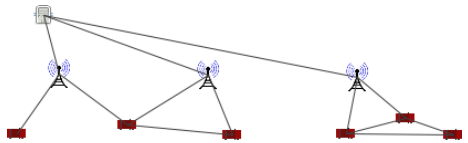
\includegraphics[width=0.7\linewidth]{fig_2}
	\caption[A highway scenario composed of vehicles, road-side units, and central servers. Part of the network is ad hoc (and wireless); the rest is infrastructured (and wired).]{A highway scenario composed of vehicles, road-side units, and central servers. Part of the network is ad hoc (and wireless); the rest is infrastructured (and wired).}
	\label{fig:fig2}
\end{figure}
\subparagraph{} $JBOTSIM$ consists of a small number of classes, the most central being Node, Link, and Topology. The contexts in which dynamic networks apply are varied. In order to accommodate a majority of cases, these classes offer a number of conceptual variations around the notions of nodes and links. Nodes may or may not possess wireless communication capabilities, sensing abilities, or self-mobility. They may differ in clock frequency, color, communication range, or any other user-defined property. Links between the nodes account for potential communication among them. The nature of links varies as well; a link can be directed or undirected, as well as it can be wired or wireless – in the latter case  $JBOTSIM$ ’s topology will update the set of links automatically, as a function of nodes distances and communication ranges.
\subparagraph{} $JBOTSIM$  consists of a small number of classes, the most cen- tral being Node, Link, and Topology. The contexts in which dynamic networks apply are varied. In order to accommodate a majority of cases, these classes offer a number of conceptual variations around the notions of nodes and links. Nodes may or may not possess wireless communication capabilities, sensing abilities, or self-mobility. They may differ in clock frequency, color, communication range, or any other user-defined property. Links between the nodes account for potential communication among them. The nature of links varies as well; a link can be directed or undirected, as well as it can be wired or wireless – in the latter case  $JBOTSIM$ ’s topology will update the set of links automatically, as a function of nodes distances and communication ranges.
\begin{figure}[h!]
	\centering
	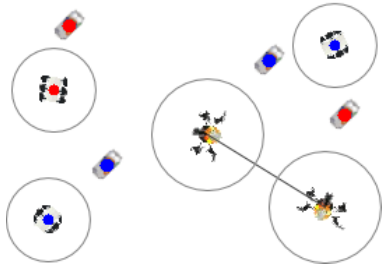
\includegraphics[width=0.7\linewidth]{fig_3}
	\caption[A swarming scenario, whereby mobiles robots and UAVs collaborate in order to clean a public park.]{A swarming scenario, whereby mobiles robots and UAVs collaborate in order to clean a public park.}
	\label{fig:fig3}
\end{figure}
Figure 2 illustrates a purely ad hoc scenario, whereby a heterogeneous swarm of UAVs and robots strives to clean a public park collectively. In this scenario, robots can detect and clean wastes of a certain type (red or blue) only if these are within their sensing range (depicted by a surrounding circle). However, they are pretty slow to move and cannot detect remote wastes. In the mean- time, a set of UAVs is patrolling over the park at higher speed and with larger sensing range. Whenever they detect a waste of some type, they store its position and start searching for a capable robot. In addition to sensing capabilities, UAVs can exchange messages with each other to optimize the process.
\subparagraph{}Besides nodes and links, the concept of topology is central in  $JBOTSIM$. Topologies can be thought of as containers for nodes and links, together with dedicated operations like updating wireless links. They also play a central role in  $JBOTSIM$ ’s event architecture, as explained later on.
\subparagraph{Distributed vs. centralized algorithms}
\subparagraph{} $JBOTSIM$  supports the manipulation of centralized or distributed algorithms (possibly simultaneously). The natural way to imple- ment a distributed algorithm is by extending the Node class, in which the desired behavior is implemented. Centralized algorithms are not constrained to a particular model, they can take the form of any standard java class.
\subparagraph{Distributed algorithm} $JBOTSIM$  comes with a default type of node that is implemented in the Node class. This class provides the most general features a node could have, including primitives for moving, exchanging messages, or tuning basic parameters (e.g. communication range and sensing range). Distributed algorithms are naturally implemented through adding specific features to this class. Listing 2 provides a basic example in which the nodes are endowed with self-mobility. The class relies on a key mechanism in  $JBOTSIM$ : performing periodic operations that are triggered by the pulse of the system clock. This is done by overriding the onClock() method, which is called periodically by JBotSim’s engine (by default, at every pulse of the clock). The rest of the code is responsible for moving the node, setting a random direction at construction time (in radian), then moving in this direction periodically. (More de- tails about the movement API can be found online.) Once this class is defined, new nodes of this type can be added to the topology in the same way as if they were of class Node, as illustrated in Listing 3. Here, a new topology is created first, then 10 nodes of the desired type (here, MovingNode) are added through the addNode() method at random locations (using -1 for x- coordinate or y-coordinate generates a random location for that co- ordinate; here both are random). In order to use MovingNode through the GUI, for instance when clicking with the mouse to add new nodes, this class must be registered as a node model. This is done by calling method setDefaultNodeModel() with the class itself as an argument, as shown on Listing 4. $JBOTSIM$ will create new instances on the fly, using reflexivity. Several models can be registered simultaneously, using setNodeModel() with an additional argument that corresponds to the model name. If several models exist,  $JBOTSIM$ ’s GUI (the viewer) displays a selection list when a node is added by the user (in this example, only one model is set and it is used by default). In the scenario of Figure 1, however, left-clicking on the surface would give the choice between car, tower, and server, the names of the three registered models for that scenario.
\begin{lstlisting} [caption=Extending the Node class,captionpos=b]
import jbotsim.Node;
public class MovingNode extends Node{
	public MovingNode(){
		setDirection(Math.random() * 2*Math.PI);
	}
	public void onClock(){
		move(2);
	}
}
\end{lstlisting}

\begin{lstlisting} [caption=Adding nodes manually,captionpos=b]
public static void main(String[] args){
	Topology tp = new Topology(400, 300); tp.setDefaultNodeModel(MovingNode.class);
	new JViewer(tp);
}
\end{lstlisting}

\begin{lstlisting}[caption=Using a defined node as default, captionpos=b]
public static void main(String[] args){
	Topology tp = new Topology(400, 300); tp.setDefaultNodeModel(MovingNode.class);
	new JViewer(tp);
}
\end{lstlisting}


\subparagraph{Centralized algorithms}There are many reasons why a centralized algorithm can be preferred over a distributed one. The object of study might be centralized in itself (e.g. network optimization, scheduling, graph algorithms in general). It may also be simpler to simulate distributed things in a centralized way. Listing 5 implements such a version of the random way-point mobility model, in which nodes repeatedly move toward a randomly selected destination, called target. Unlike a distributed implementation, the movements of nodes are here driven by a global loop at every pulse of the clock. For each node, a target is created if it does not exists yet or if it has just been reached; then the node’s direction is set accordingly and the node is moved (by default, by 1 unit of distance). For convenience, the main() method is included in the same class. Notice the use of setProperty() and getProperty() in this example. These methods allow to store any object directly into a node, using a key/value scheme (where key is a string). Both Link and Topology objects offer the same feature.
\subparagraph{Architecture of the event system}
So far, we have seen one type of event: clock pulses, to be listened to through the ClockListener interface. $JBOTSIM$ offers a number of such events and interfaces, some of which become are ubiquitous. The main ones are depicted on Figure 3 on the fol- lowing page. This architecture allows one to specify dedicated operations in reaction to various events. For instance, one may ask to be notified whenever a link appears or disappears somewhere. Same for messages, which are typically listened to by the nodes themselves or can be watched at a global scale (e.g. to keep a log of all communications). In fact, every node is automatically notified for its own events; it just needs to override the corresponding methods from the parent class Node in order to specify event handlings (e.g. onClock(), onMessage(), onLinkAdded(), onSensingIn(), onSelection(), etc.). Explicit listeners, on the other hand, like the ones in Figure 3, are meant to be used by centralized programs which do not extend class Node. Listing 6 gives one such example, consisting of a mobility trace recorder. This program listens to topological events of various kinds, including appearance or disappearance of nodes or links, and movements of the nodes. Upon each of these events, it outputs a string representation of the event using a dedicated human readable format called DGS [7]. Similar code could be written for Gephi [3]. Other events exist besides those represented in Figure 3, such as the SelectionListener interface, which makes it possible to be notified when a node is selected (middle-click) and make it initiate some tasks, for instance broadcast, distinguished role, etc.
\subparagraph{Single threading: why and how?}It seems convenient at first, to assign every node a dedicated thread, however $JBOTSIM$ was designed differently. $JBOTSIM$ is single-threaded, and definitely so. This section explains the why and the how. Understanding these aspects are instrumental in developing well-organized and bug-free programs.
\begin{figure}[h!]
	\centering
	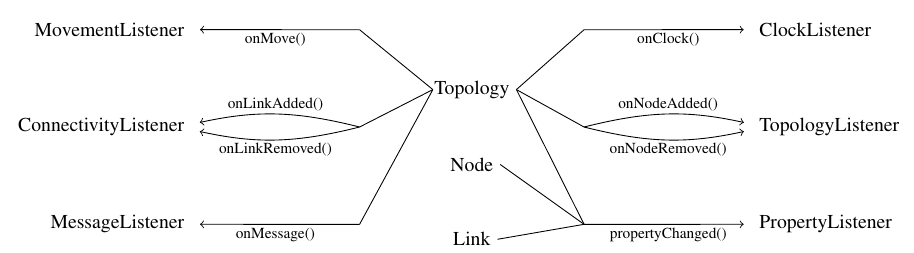
\includegraphics[width=1\linewidth]{fig_4}
	\caption[Main sources of events and corresponding interfaces in  $JBOTSIM$ .]{Main sources of events and corresponding interfaces in  $JBOTSIM$ .}
	\label{fig:fig4}
\end{figure}

\begin{lstlisting}[caption=Centralized version of Random Waypoint, captionpos=b]
public class MyRecorder implements TopologyListener, ConnectivityListener, MovementListener{
	public MyRecorder(Topology tp){
		tp.addTopologyListener(this);
		tp.addConnectivityListener(this);
		tp.addMovementListener(this);
	}
	// TopologyListener
	public void onNodeAdded(Node node) {
	 	println("an " + node.hashCode() +
	 		" x:" + node.getX() + " y:" + node.getY());
	 }
	 
	 public void onNodeRemoved(Node node) {
	 	println("dn " + node.hashCode());
	 }
	 // ConnectivityListener
	 public void onLinkAdded(Link link) {
	 	println("ae " + link.hashCode() + " " +
	 		link.endpoint(0) + " " + link.endpoint(1));
	 }
	 public void onLinkRemoved(Link link) {
	 	println("de " + link.hashCode());
	 }
	 // MovementListener
	 public void onNodeMoved(Node node) {
	 	println("cn " + node.hashCode() +
	 		" x:" + node.getX() + " y:" + node.getY());
	 	}
	 }
\end{lstlisting}
\subparagraph{}In  $JBOTSIM$ , all the nodes, and in fact all of  $JBOTSIM$ ’s life (GUI excepted) is articulated around a single thread, which is driven by the central clock. The clock pulses at regular interval (whose period can be tuned) and notifies its listeners in a specific order.  $JBOTSIM$ ’s internal engines, such as the message engine, are served first. Then come those nodes whose wait period has expired (re- mind that nodes can choose to register to the clock with different periods). These nodes are notified in a random order. Hence, if all nodes listen to the clock at a rate of 1 (the default value), they will all be notified in a random order in each round, which makes  $JBOTSIM$ ’s scheduler a non-deterministic 2-bounded fair sched- uler. (Other policies will be available eventually.) A simplified version of the current scheduling process is depicted on Figure 4.
\subparagraph{}One consequence of single-threading is that all computations (GUI excepted) take place in a sequential order that makes it possible to use unsynchronized data structures and simpler code. This also improves the scalability of $JBOTSIM$ when the number of nodes grows large. One can rely on other user-defined threads in the program, however one should be careful that these thread do not interfer with  $JBOTSIM$ ’s. The canonical example is when a scenario is set up by program from within the thread of the main() method. If the initialization makes extensive use of  $JBOTSIM$ ’s API from within that thread and the clock starts triggering events at the same time, then problems might occur (and a Concurrent ModificationException be raised). The easy way around is to pause the clock before executing these instructions and to resume it after (using the pause() and the resume() methods on the topology, respectively).
\begin{figure}[h!]
	\centering
	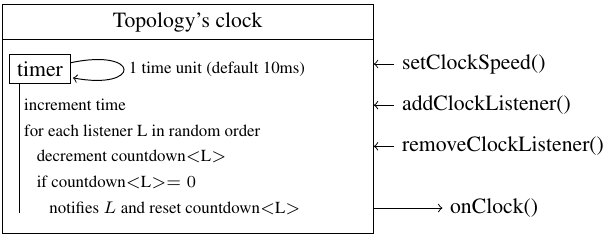
\includegraphics[width=.7\linewidth]{fig_5}
	\caption[Simplified version of the internal scheduler.]{Simplified version of the internal scheduler.}
	\label{fig:fig5}
\end{figure}
\subparagraph{Interactivity}I designed $JBOTSIM$ with a clear separation in mind between GUI and internal features. In particular, it can be run without GUI (i.e. without creating the JViewer object), and things will work exactly the same, though invisibly. As such, $JBOTSIM$ can be used to perform batch simulations (e.g. sequences of unattended runs that log the effects of some varying parameter). This also enables to withstand heavier simulations in terms of the number of nodes and links.
\subparagraph{}This being said, one of the most distinctive features of $JBOTSIM$ remains interactivity, e.g., the ability to challenge the algorithm in difficult configurations through adding, removing, or moving nodes during the execution. This approach proves useful to think of a problem visually and intuitively. It also makes it possible to explain someone an algorithm through showing its behavior.
\subparagraph{}The architecture of  $JBOTSIM$ ’s viewer is depicted on Figure 5. As one can see, the viewer relies heavily on events related to nodes, links, and topology. The influence also goes the other way, with mouse actions being translated into topological operations. These features are realized by a class called JTopology. This class can often be ignored by the developer, which creates and manipulates the viewer through the higher JViewer class. The latter adds external features such as tuning slide bars, popup menus, or self-containment in a system window. 
\subparagraph{}While natural to  $JBOTSIM$ ’s users, the viewer remains, in all technical aspects, an independent piece of software. Alternative viewers could very well be designed with specific uses in mind.

\begin{figure}[h!]
	\centering
	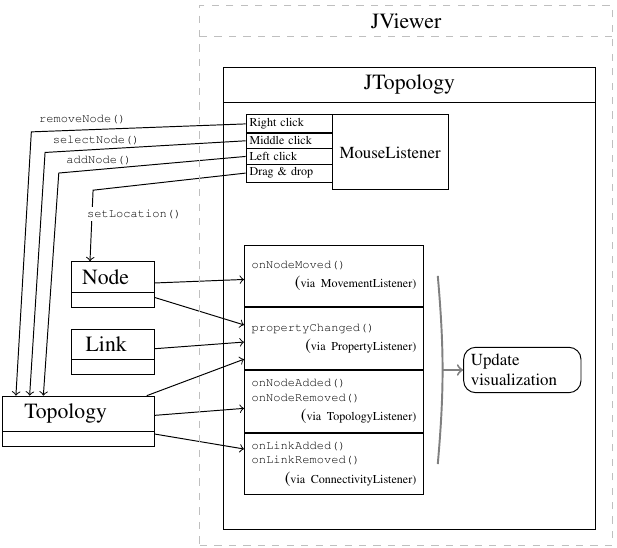
\includegraphics[width=.7\linewidth]{fig_6}
	\caption[Internals of JBotSim’s GUI]{Internals of JBotSim’s GUI}
	\label{fig:fig6}
\end{figure}
\paragraph{A zoom on selected features}This section provides more details on a handful of selected features. It covers, namely, the topics of message passing, graph-level algorithms, and java applets for online web demos.
\subparagraph{Exchanging messages}The way messages are used in $JBOTSIM$ is independent from the communication technology considered. Indeed, the API is quite simple, messages are sent directly by the sender, through calling the send() method on its own instance (inherited from Node). Messages are typically received through overriding the onMessage() method (also from class Node). Another way to receive messages, which is not event-based, is for a node to check its mailbox manually through the getMailbox() method, for instance when it is executing the onClock() method (this is the natural way to implement round-based communication models). \subparagraph{}Listing 7 shows a message-based implementation of the flooding principle. Initially, none of the nodes are informed. Then, if a node is selected (either through middle-click or through direct call to the selectNode() method), then this node is notified in the onSelection() method and initiates a basic broadcast scheme. Here, the algorithm consists in retransmitting the received message upon first reception to all the local neighbors (sendAll()). In this example, the message is empty, however in general any object can be inserted in the message (no copy is made and the very same object is to be delivered, unless a copy is made at sending time). By default, a message takes one time unit to be transmitted (i.e. it is delivered at the next clock pulse). The delivery happens only for those links which exist by the time of reception. Since any object can be used as message content, it often has to be cast upon reception. All these aspects correspond to  $JBOTSIM$ ’s default message engine. Other message engines can be written, and indeed some exist in the jbotsimx package. For instance, the DelayMessageEngine makes it possible to add deterministic or random delays to the delivery of messages, possibly even in a non FIFO manner.
\subparagraph{Working at the graph level}
\begin{lstlisting}[caption=Example of message passing algorithm, captionpos=b]
public class FloodingNode extends Node{
	boolean informed = false;
	@Override 
	public void onSelection() {
		informed = true;
		sendAll(new Message());
	}
	@Override
	public void onMessage(Message message) {
		if (!informed){
			informed = true;
			sendAll(message);
		}
	}
}
\end{lstlisting}
\subparagraph{}Implementing an algorithm in the message passing model is some- times difficult. $JBOTSIM$ makes it possible to sketch an idea, play with it, and share it with others, in minutes, thanks to working at a (more abstract) graph-level. This level of abstraction also is relevant in its own right, when the object of study is itself at the graph level, such as classical graph algorithms or distributed coarse-grain models like graph relabeling systems [9] or population protocols [2].
\subparagraph{}To illustrate the simplicity of the graph level, let us consider a scenario where a type of node called SocialNode, dislikes being isolated. Such a node is happy (green) if it has at least one neighbor, unhappy (red) otherwise. In the message passing paradigm, this principle would require to send periodic messages (beacons) and track the reception of these messages, as well as using a timer to decide when a node becomes isolated. Listing 8 shows a possible implementation at the graph level, which is pretty concise and self-explanatory. Topological events are directly detected by the nodes, which can update their status. (These events could also be listened to globally through the ConnectivityListener() interface. This is the way one might want to implement centralized dynamic graph algorithms.) Of course, from a message passing perspective, this implementation is cheating. Thus, methods like onLinkAdded(), hasNeighbors(), or getNeighbors() should not be used in a message-passing setting.

\begin{lstlisting}[caption=Example of graph-based algorithm, captionpos=b]
public class SocialNode extends Node{
	public SocialNode(){
		setColor(Color.red);
	}
	public void onLinkAdded(Link l){
		setColor(Color.green);
	}
	public void onLinkRemoved(Link l){
		if (!hasNeighbors())
			setColor(Color.red);
		}
	}
\end{lstlisting}
\subparagraph{Embedding JBOTSIM in a java applet}One of the features of  $JBOTSIM$ ’s viewer is to create a windowed frame automatically for the topology. This is the default behavior of JViewer’s constructor when a single parameter of type Topology or JTopology is used. Other behaviors can be obtained by using different versions of the constructor. In particular, one can specify that no windowed frame should be created, and the JTopology object be plugged manually into a different container. This feature enables the customization of  $JBOTSIM$ ’s UI at will, as well as the creation of java applets.
\subparagraph{}Listing 9 shows an example java applet corresponding to the HelloWorld program from Listing 1. Here, a JTopology object (which is a JPanel) is created manually from the topology. Its reference is then used to augment it with standard viewer features, and finally added to the applet container. Another important step is to pause the clock in the destroy() method (otherwise JBotSim’s engine would keep running in background).

\begin{lstlisting}[caption=Embedding a $JBOTSIM$ demo into a java applet, captionpos=b]
import javax.swing.JApplet;
import jbotsim.Clock;
import jbotsim.Topology;
import jbotsim.ui.JTopology;
import jbotsim.ui.JViewer;
@SuppressWarnings("serial")
public class HelloWorld_Applet extends JApplet{
	Topology tp;
	public void init(){
		tp = new Topology();
		JTopology jtp = new JTopology(tp);
		new JViewer(jtp, false);
		this.add(jtp);
	}
	public void destroy(){
		tp.pause();
	}
}
\end{lstlisting}

\paragraph{Concluding remarks}I my view, $JBOTSIM$ is a kernel, in the sense that it encapsulates a number of generic features whose purpose is to be used by higher programs. As of today, the plan is to keep it this way and try containing the growth of the number of features, to the profit of quality and simplicity. This does not mean, of course, that JB OT- S IM should not be extended externally.
\paragraph{}In particular,  $JBOTSIM$’s distribution already incorporates an ex- tension package called jbotsimx, in which more specific features could be found. For instance, it incorporates a static class called Tikz that makes it possible to export the current topology as a TikZ picture – a powerful format for drawing pictures in LATEX documents. Figure 6 illustrates this with two pictures that I have generated. The Tikz class is composed of a single method, exportAsTikz(), which takes a mandatory Topology argument, and an optional scaling argument.
\paragraph{}Other extensions include basic topology algorithms for testing, e.g., if a given topology is connected or 2-connected, if a given node is critical (its removal would disconnect the graph) or compute the diameter. A set of extensions dedicated to dynamic graph are currently being developed (by myself and others). For instance, the EMEGPlayer takes as input a birth rate, death rate, and an underlying graph (given as a Topology), and generates an edge-markovian dynamic graph based on these parameters, the dynamics of which can be listened to through the ConnectivityListener interface.
\paragraph{}Contributions are most welcome, as well as suggestions of improvement or feature requests.

\begin{figure}[h]
	\centering
	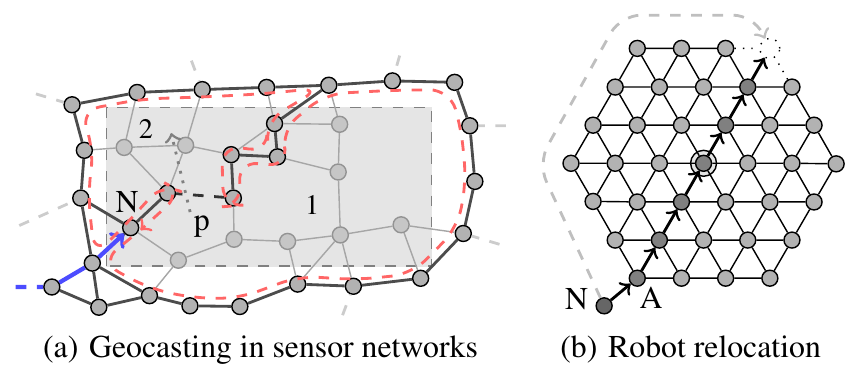
\includegraphics[width=0.7\linewidth]{fig_7}
	\caption[Two examples of pictures whose underlying topology was generated using $JBOTSIM$ Tikz extension. The topology on the left was created by adding and moving nodes using the mouse; the topology on the right was generated by program. Once exported as a Tikz picture, they were twicked manually to add shading, color, etc.]{Two examples of pictures whose underlying topology was generated using $JBOTSIM$ Tikz extension. The topology on the left was created by adding and moving nodes using the mouse; the topology on the right was generated by program. Once exported as a Tikz picture, they were twicked manually to add shading, color, etc.}
	\label{fig:fig7}
\end{figure}


\section{Performance Analysis}

This section presents performance characteristics of our algorithm measured through simulations using JBOTSIM\cite{26} tool. We consider the following metrics defined for any component of size $n$.

\begin{enumerate}
	\item \textbf{Latency} $l$. The number of rounds necessary for a component to elect a leader (become stable) after a topology change (average over all initial topologies).
	
	\item \textbf{Sensitivity} $s$. The number of nodes that updated their heights in response to a topology change (average over all possible topology changes).
	
	\item \textbf{Resilience} $r$. The maximal fraction of links which can go down in a stable component without reelecting the current leader.
	
\end{enumerate}

We have measured these parameters using simulations of several scenarios (Figures 6(a) and 6(b)), and we summarize them below:

\begin{itemize}
	\item Merging two stable components:
	
	\begin{itemize}
		\item Given two fully connected (every two nodes are neighbours) components: $l \simeq 2$.
		\item Given two poorly connected (a node can have not more than two neighbours) components: $l \simeq n$.
	\end{itemize}
	
	\item Partitioning a stable component:
	
	\begin{itemize}
		\item Getting two fully connected component: $l = 2$.
		\item Getting two poorly connected component: $l = 2n$.
	\end{itemize}
	
	\item Topology change in a “small world-like” stable component (every node has $O(log n)$ neighbours) without partitioning:
	\begin{itemize}
		\item Latency $l$ = $O(1)$.
		\item Sensitivity $s$ = $O(log(n))$.
	\end{itemize}
	
	\item Resilience of a stable component:
	
	\begin{itemize}
		\item Given a fully connected component: $r \approx 1 - 2/n$.
		\item Given a “small world-like” component: $r \approx 1 - 2/log(n)$.
	\end{itemize}
	
\end{itemize}


\begin{figure}[hbtp]
	\centering
	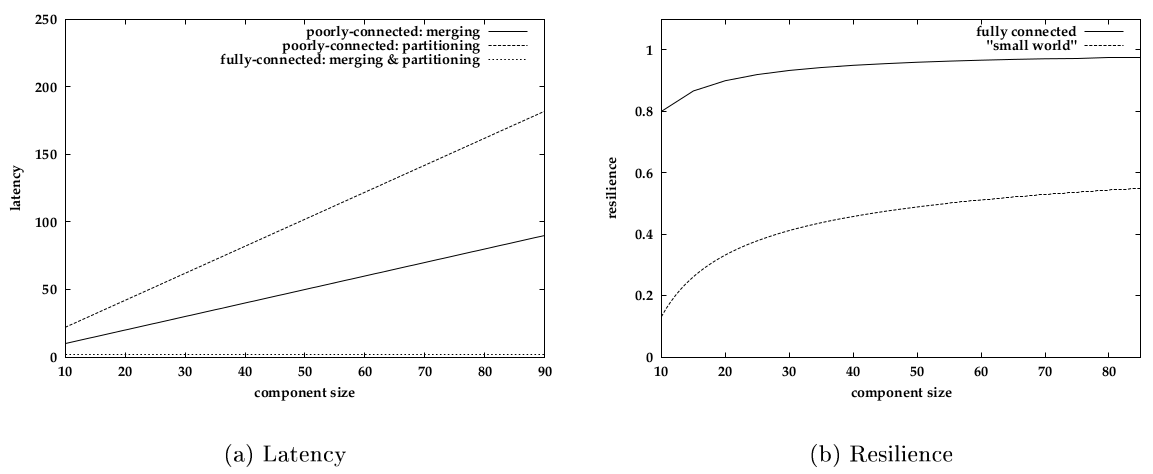
\includegraphics[scale=.4]{performance_test.png}
	\caption{Simulation results}
\end{figure}

\chapter{Sample Title}

Lorem ipsum dolor sit amet, consectetur adipiscing elit, sed do eiusmod tempor incididunt ut labore et dolore magna aliqua. Ut enim ad minim veniam, quis nostrud exercitation ullamco laboris nisi ut aliquip ex ea commodo consequat. Duis aute irure dolor in reprehenderit in voluptate velit esse cillum dolore eu fugiat nulla pariatur. Excepteur sint occaecat cupidatat non proident, sunt in culpa qui officia deserunt mollit anim id est laborum.

%now enable appendix numbering format and include any appendices


%next line adds the Bibliography to the contents page
\addcontentsline{toc}{chapter}
{Bibliography}
%uncomment next line to change bibliography name to references
%\renewcommand{\bibname}{References}
\bibliography{refs}        %use a bibtex bibliography file refs.bib
\bibliographystyle{plain}  %use the plain bibliography style

\end{document}

